\documentclass[11pt]{article}

\usepackage{booktabs} % For formal tables
\usepackage{tikz} % SW: Added for plots

\usepackage{fullpage}
\usepackage{kpfonts}
 \usepackage{url}

% call this *before* "algorithm2e"
\usepackage[round]{natbib}


\usepackage[ruled]{algorithm2e} % For algorithms
\renewcommand{\algorithmcfname}{ALGORITHM}
\SetAlFnt{\small}
\SetAlCapFnt{\small}
\SetAlCapNameFnt{\small}
\SetAlCapHSkip{0pt}
\IncMargin{-\parindent}


\usepackage{amsmath, amsthm, amssymb}
%\usepackage{natbib}
%\usepackage{cleveref}
\usepackage{slivkins-setup}

\definecolor{DarkGreen}{rgb}{0.1,0.5,0.1}
\definecolor{DarkRed}{rgb}{0.5,0.1,0.1}
\definecolor{DarkBlue}{rgb}{0.1,0.1,0.5}
\usepackage[]{hyperref}
\hypersetup{
    unicode=false,          % non-Latin characters in Acrobat's bookmarks
    pdftoolbar=true,        % show Acrobat toolbar?
    pdfmenubar=true,        % show Acrobat menu?
    pdffitwindow=false,      % page fit to window when opened
    pdftitle={},    % title
    pdfauthor={}
    pdfsubject={},   % subject of the document
    pdfnewwindow=true,      % links in new window
    pdfkeywords={keywords}, % list of keywords
    colorlinks=true,       % false: boxed links; true: colored links
    linkcolor=DarkRed,          % color of internal links
    citecolor=DarkGreen,        % color of links to bibliography
    filecolor=DarkRed,      % color of file links
    urlcolor=DarkBlue,          % color of external links
}

\newtheorem{theorem}{Theorem}[section]
\newtheorem{claim}[theorem]{Claim}
% \theoremstyle{remark}
\newtheorem{remark}[theorem]{Remark}
\newtheorem{corollary}[theorem]{Corollary}
\newtheorem{lemma}[theorem]{Lemma}
\newtheorem{definition}[theorem]{Definition}




% a very useful package for edits and comments, from David Kempe (USC)
\usepackage{color-edits}
%\usepackage[suppress]{color-edits}  % use this to suppress the package
\addauthor{as}{red}      % as for Alex
\addauthor{ym}{blue}    % ym for Yishay
\addauthor{sw}{cyan}   % sw for Steven
% e.g. for Alex, provides \asedit{}, \ascomment{} and \asdelete{}.
\newcommand{\sw}[1]{\swcomment{#1}} % for compatibility with Steven's macro


\DeclareMathOperator*{\Expectation}{\mathbb{E}}
\newcommand{\Ex}[2]{\Expectation_{#1}\left[#2\right]}


% notation
%%% advanced notation
\newcommand{\term}[1]{\ensuremath{\mathtt{#1}}\xspace}
\newcommand{\OPT}{\term{OPT}}
\newcommand{\rew}{\term{rew}}  % Bayesian-expected reward after n local rounds
\newcommand{\PMR}{\term{PMR}} % posterior mean reward
\newcommand{\support}{\term{support}}

\newcommand{\BIR}{\term{BIR}} % Bayesian Instantaneous Regret
\newcommand{\regret}{R^{\term{inst}}} % regret
\newcommand{\regretWC}{\regret_{\term{wc}}} % regret

% response function
\newcommand{\respF}{f_{\term{resp}}}
\newcommand{\respEps}{\eps_\term{resp}}

\newcommand{\HardMax}{\term{HardMax}}
\newcommand{\HardMaxRandom}{\term{HardMax\&Random}}
\newcommand{\SoftMaxRandom}{\term{SoftMax}}
\newcommand{\Uniform}{\term{Uniform}}
\newcommand{\Random}{\term{Random}}

\newcommand{\StaticGreedy}{\term{StaticGreedy}}
\newcommand{\DynGreedy}{\term{DynamicGreedy}}
\newcommand{\DynamicGreedy}{\term{DynamicGreedy}}

\newcommand{\termSub}[2]{\ensuremath{\mathtt{#1}_{#2}}\xspace}
\newcommand{\alg}[1][]{\termSub{alg}{#1}}
%\newcommand{\prin}[1][]{\termSub{prin}{#1}}  % principal
\newcommand{\agent}[1][]{\termSub{agent}{#1}}

% priors and posteriors
\newcommand{\prior}{\ensuremath{\mP}\xspace}
\newcommand{\priorMu}{\ensuremath{\prior_\mathtt{mean}}\xspace}
\newcommand{\posteriorN}[2]{\mN_{#1,#2}}  % \posteriorN{principal}{round}

% rationality / innovation / competition
\newcommand{\termTXT}[1]{{\em {#1}}\xspace}

\newcommand{\rationality}{\termTXT{rationality}}
\newcommand{\Rationality}{\termTXT{Rationality}}
\newcommand{\innovation}{\termTXT{innovation}}
\newcommand{\Innovation}{\termTXT{Innovation}}
\newcommand{\competition}{\termTXT{competition}}
\newcommand{\Competition}{\termTXT{Competition}}
\newcommand{\exploration}{\termTXT{exploration}}
\newcommand{\Exploration}{\termTXT{Exploration}}

\begin{document}
\title{Competing Bandits: Learning under Competition}


\author{Yishay Mansour\thanks{Tel Aviv University. Email: mansour@tau.ac.il}
 \and Aleksandrs Slivkins\thanks{Microsoft Research-New York City. Email: slivkins@microsoft.com}
 \and Zhiwei Steven Wu\thanks{University of Pennsylvania. Email: wuzhiwei@cis.upenn.edu} }

\date{February 2017}


\maketitle

% abstract must come before \maketitle
\begin{abstract}
Most modern systems strive to learn from interactions with users, and many engage in \emph{exploration}: making potentially suboptimal choices for the sake of acquiring new information. We initiate a study of the interplay between \emph{exploration and competition}---how such systems balance the exploration for learning and the competition for users. Here the users play three distinct roles: they are customers that generate revenue, they are sources of data for learning, and they are self-interested agents which choose among the competing systems.

In our model, we consider competition between two multi-armed bandit algorithms faced with the same bandit instance. Users arrive one by one and choose among the two algorithms, so that each algorithm makes progress if and only if it is chosen.
%We ask whether better algorithms perform better in such competition,
% and whether the competition incentivizes better algorithms
% and improves social welfare.
We ask whether and to what extent competition incentivizes \asedit{the adoption of better bandit algorithms}. We investigate this issue for several models of user response, as we vary the degree of rationality and competitiveness in the model. \asedit{Our findings are closely related to} the ``competition vs. innovation" relationship, a well-studied theme in economics.



\end{abstract}


\section{Introduction}
\label{sec:intro}

Learning from interactions with users is ubiquitous in modern customer-facing systems, from product recommendations to web search to content selection to fine-tuning user interfaces. Many systems purposefully implement \emph{exploration}: making potentially suboptimal choices for the sake of acquiring new information.
Online platforms routinely deploy A/B tests, and are increasingly adopting  more sophisticated exploration methodologies based on \emph{multi-armed bandits}, a well-known framework for exploration and making decisions under uncertainty. 


%~\cite{KohaviAB-2015,KohaviLSH09}

In this paper, we initiate a study of the interplay between \exploration and \competition. Systems that engage in exploration typically need to compete against one another; most importantly, they compete for users. This creates a tension:
%between \exploration and \competition. 
while exploration may be essential for improving the service tomorrow, it may degrade quality and make users leave \emph{today}, in which case there will be less users to learn from. This may further degrade the platform's performance relative to competitors who keep learning and improving from \emph{their} users, and so forth. Taken to the extreme, such dynamics may create a ``death spiral" effect when the vast majority of customers eventually switch to competitors. Users therefore serve three distinct roles: they are customers that generate revenue, they are sources of data for learning, and they are self-interested agents who choose among the competing systems.

\ascomment{stopped here.}

The main high-level question that we focus on in this paper is whether competition between systems incentives the adoption of better exploration algorithms. This translates into a number of more concrete questions. While it is commonly assumed that ``better" technology always helps, is this so for our setting? Does increasing competition lead to higher consumer welfare? To what extent is there a ``data feedback loop" where one firm having more data leads to that firm attracting more users which leads to that firm having more data, etc.?\footnote{This is a fundamental question which is part of a larger policy discussion around whether data can serve as an indirect network effect and lead to similar ``market tipping" results as is standard in the literature on competition in markets with network effects (see \cite{jullien2019economics} for a policy oriented discussion of this).}

% the extent to which the game between the two principals is competitive
% degree of innovation that these models incentivize.
% the extent to which agents make rational decisions


%\subsection{Our model}
%\label{sec:intro-model}

\xhdr{Our model.} We investigate these questions with a stylized duopoly model where two firms commit to exploration strategies and compete for a stream of consumers. We define a game in which two firms (\emph{principals}) simultaneously engage in exploration and compete for users (\emph{agents}). These two processes are interlinked, as exploration decisions are experienced by users and informed by their feedback. We need to specify several conceptual pieces: how the principals and agents interact, what is the machine learning problem faced by each principal, and what is the information structure. Each piece can get rather complicated in isolation, let alone jointly, so we strive for simplicity. Thus, the basic model is as follows:

\begin{itemize}

\item A new agent arrives in each round $t=1,2, \ldots$, and chooses among the two principals. The principal chooses an action (\eg a list of web search results to show to the agent), the user experiences this action, and reports a reward. All agents have the same ``decision rule" for choosing among the principals given the available information.

\item Each principal faces a very basic and well-studied version of the multi-armed bandit problem: for each arriving agent, it chooses from a fixed set of actions  (a.k.a. \emph{arms}) and receives a reward drawn independently from a fixed distribution specific to this action.

\item Principals simultaneously announce their learning algorithms before round $1$, and cannot change them afterwards. There is a common Bayesian prior on the rewards (but the realized reward distributions are not observed by the principals or the agents).  Each principal only observes agents that chose him. We consider two variants of the baseline model and the information set for the agent differs between the two:
\begin{enumerate}
\item In the \textit{expectation choice variant}, agents do not receive any other information and choose between the principals using their knowledge of $t$ and the principals' algorithms.
\item In the \textit{reputation choice variant}, agents have access to a reputation score for each principal, which is a sliding window average of the rewards experienced by previous agents that have visited this principal.
\end{enumerate}
\end{itemize}

\xhdr{Main Findings.}
We find that competition induces firms to commit to a greedy (myopic) algorithm in equilibrium that does no purposeful exploration. This leads to low consumer welfare since the greedy algorithm is known to be dramatically bad in many important cases of multi-armed bandits. The primary mechanism that generates this stark result is that consumers need to be incentivized to select a firm over its competitors, leading a firm that engages in exploration to be starved of consumers before it makes enough progress on its learning problem. In order to incentivize ``better" exploration strategies in equilibrium, the key intuition is that the firm needs to have some ``free" consumers that visit them without the firm having to incentivize them to do so. This allows the firm to eventually overcome the initial losses in consumer perception from exploration. We explore two economic mechanisms that can generate such an effect.

The first is the presence of users who randomly choose between the firms which gives each firm a constant stream of ``free" users and thus ensures it never gets fully starved. We find that, even when there is a small fraction of such consumers, better algorithms help in a big way: a sufficiently better algorithm is guaranteed to win all non-random agents after an initial learning phase.\footnote{While the precise notion of ``sufficiently better algorithm" is rather subtle, we note that commonly known ``smart" bandit algorithms typically defeat the commonly known ``naive" ones, and the latter typically defeat the greedy algorithm. However, there is a substantial caveat: one can defeat any algorithm by interleaving it with the greedy algorithm. This has two undesirable corollaries: a better algorithm may sometimes lose, and a pure Nash equilibrium typically does not exist.} However, while this holds asymptotically, our numerical experiments show that this requires either unreasonably large time scales or a large fraction of such users.

The second is that if one firm has a first-mover advantage then this firm gets free users before the other firm enters into the market. We show that if this incumbency period is sufficiently long, then it allows the firm to make sufficient progress on its learning problem and incentivizes it to commit to better algorithms. While this leads to the incumbent getting almost all of the market, it leads to higher consumer welfare than under competition when the firms enter at the same time.

\xhdr{\underline{Additional Findings}}

\xhdr{Reputation and Data Advantage}: In the reputation choice variant we investigate the first-mover advantage phenomenon in more detail. Being first in the market gives the incumbent free data to learn from (a ``data advantage") as well as a more definite, and possibly better reputation compared to an entrant (a ``reputation advantage"). We run additional experiments so as to isolate and compare these two effects. We find that either effect alone leads to a significant advantage under competition. The data advantage is larger than reputation advantage when the incumbent commits to a more advanced bandit algorithm. This result shows that even a small amount ``data advantage" gets amplified under competition, causing a large difference in eventual market shares.

\xhdr{Noise in consumer choice}: We further relax the decision rule of the agents so that the probability of choosing a given firm varies smoothly as a function of the difference between  principals' expected rewards. For this decision rule, the ``better algorithm wins" result holds under much weaker assumptions on what constitutes a better algorithm. This is the most technical result of the paper. The competition in this setting is necessarily much more relaxed: typically, both principals attract approximately half of the agents as time goes by (but a better algorithm may attract slightly more).

\xhdr{Predicting Outcomes in Competition} We also investigate how algorithms' performance ``in isolation" (without competition) is predictive of the outcomes under competition in the reputation choice variant. We find that mean reputation -- arguably, the most natural performance measure ``in isolation" -- is sometimes not a good predictor. We suggest a more refined performance measure, based on a comparison between the reputation of the two firms, and use it to explain some of the competition outcomes.
\textbf{Add some discussion about comparison with ``better" algorithms in analytical part}

\OMIT{All results extend to a much more general version of the multi-armed bandit problem in which the principal may observe additional feedback before and/or after each decision, as long as the feedback distribution does not change over time. In most results, principal's utility may depend on both the market share and agents' rewards.
}

\begin{figure}
\begin{center}
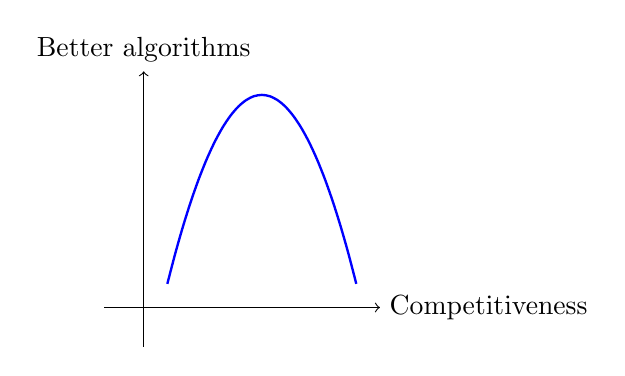
\begin{tikzpicture}
      \draw[->] (-.5,0) -- (3,0) node[right] {Competitiveness};
      \draw[->] (0,-.5) -- (0,3) node[above] {Better algorithms};
      \draw[scale=0.6,domain=0.5:4.5,smooth,variable=\x,blue, line width=0.3mm] plot ({\x},{4.5 - (\x - 2.5)^2});
      % \draw[scale=0.5,domain=-3:3,smooth,variable=\y,red]  plot ({\y*\y},{\y});
 \end{tikzpicture}

\caption{Inverted-U relationship between competitiveness and algorithms.}
\label{fig:inverted-U}
\end{center}
\end{figure}
\xhdr{Economic interpretation.} Our model speaks to two distinct strands of the economics literature.

The first is the literature that studies the relationship between competition and innovation where, in our context,  the choice between different algorithms is interpreted as firms determining whether to invest in a ``better" technology as the degree of competition varies.\footnote{The choice of algorithms has a clear analogue to ``innovation" in our context as the literature on multi-armed bandits has identified distinct ``classes" of algorithms according to asymptotic regret bounds. Thus, choosing algorithms in ``better" classes corresponds with innovation on the part of the firm in our interpretation of the model. It is not salient whether similar ideas and/or technologies already exist outside the firm. It is worth noting that the adoption of exploration algorithms tends to require substantial R\&D effort in practice, even if the algorithms themselves are well-known in the research literature; see \citet{MWT-WhitePaper-2016} for an example of such R\&D effort.} A classic result in this literature is that there is an inverted-U relationship between the severity of competition among firms and the quality of technologies that they adopt is a familiar theme in the economics literature \citep[\eg][]{Aghion-QJE05,Vives-08}.

We find it illuminating to frame our contributions in a similar manner, as illustrated in \reffig{fig:inverted-U}. In our model we consider varying the intensity of competition as varying the degree to which a firm needs to incentivize users to visit them. Competition is less intense when there are more ``random" users or one firm has a sufficiently long first-mover advantage. The inverted-U relationship in our model arise for a fundamentally different reason, compared to the existing literature on ``competition vs. innovation.'' In the literature, better technology always helps in a competitive environment, other things being equal. Thus, the trade-off is between the costs of improving the technology and the benefits that the improved technology provides in the competition. Meanwhile, we find that a better exploration algorithm may sometimes perform much worse under competition, even in the absence of R\&D costs. This stems from the nature of exploration technologies in online markets which rely on learning from interactions with users. This leads to an implicit cost from exploration in the form of a reduced rate of users that a firm attracts and can learn from.

Interestingly, the economic mechanism in our model for incentivizing firms to engage in R\&D has a qualitative similarity to the role that patents play in incentivizing innovation in standard R\&D models. In these models, patents temporarily relax competition for the innovating firm by giving them exclusive access to their innovation for a limited period of time in order to incentivize them to invest in the better technology. In our model, temporarily relaxing competition in the form of giving firms free periods to learn incentivizes the firm to invest in the better technology.

The second is the nascent literature which studies the economics of data and how data can serve as a barrier to entry in the digital economy \cite{de2020data, hagiu2020data}. Our model directly speaks to this literature as we endogenize data-driven network effects by explicitly considering a model where firms are simultaneously solving a machine learning problem while competing against each other for users. The results of our model point to the fact that competition dynamics -- that firms compete as they learn over time and that this competition endogenously determines the data observed by firms -- are pertinent to understanding whether or not data can serve as a barrier to entry. Indeed, our results are similar to the market tipping results in the literature on indirect network effects and show a channel through which differences in data ownership can result in market tipping. However, it is important to note that the channel through which this arises in our model is not simply from differences in the quantity of data possessed by the firms, but also from the quality of the data.

\xhdr{Discussion}
We consider two separate variants of the model in order to provide a more thorough investigation of the tension between exploration and competition. The expectation choice model is tractable enough to allow us to obtain theoretical results with ``asymptotic" flavor. However, for the sake of analytical tractability, we make the unrealistic simplification that users do not observe any signals about firms' ongoing performance and it is difficult to analyze important economic mechanisms such as asymmetries in the timing of entry.

The reputation choice model relaxes this simplification and accounts for competition in a more direct way as well as allows us to explore other relevant economic mechanisms in understanding the tension between exploration and competition. However, it now becomes considerably harder to analyze analytically. This is for several reasons: intricate feedback loop from performance to reputations to users to performance;
%
mean reputation, most connected to our intuition, is sometimes a bad predictor in competition (see Sections~\ref{sec:isolation} and~\ref{sec:revisited});
%
mathematical tools from regret-minimization would only produce ``asymptotic" results, which do not seem to suffice. We therefore analyze our model using numerical simulation, which has several benefits. It allows us to analyze our model from a ``non-asymptotic" perspective, looking for substantial effects within relevant time scales. Indeed, we start our investigation by determining what time scales are relevant in the context of this variant of the model. Further, it allows us to investigate important economic mechanisms that arise in environments where exploration and competition tensions are at play, such as the effect of incumbency, increasing the number of firms, and the extent to which data can serve as a barrier to entry.

\xhdr{Map of the paper.}
We survey related work (Section~\ref{sec:related-work}), lay out the model and preliminaries (Section~\ref{sec:model}). We start by analyzing the expectation choice model analytically. In Sections ~\ref{sec:rational},~\ref{sec:random}, and ~\ref{sec:soft} we analyze the expectation choice variant and characterize the equilibrium behavior under three different agent decision rules. Then, we turn to analyze the reputation choice variant of the model with details of the analysis described in Section ~\ref{sec:sim_details}. Sections ~\ref{sec:isolation} and ~\ref{sec:revisited} overview results from running different bandit algorithms in isolation (i.e. without competition). Sections ~\ref{sec:competition} and ~\ref{sec:barriers} overview the results of the reputation choice variant. Section ~\ref{sec:non_greedy} presents results of varying the consumer choice rule in the reputation choice variant. Section ~\ref{sec:conclusion} concludes.


%%% Local Variables:
%%% mode: latex
%%% TeX-master: "main"
%%% End:


\section{Related work}
\label{sec:related-work}
Multi-armed bandits (\emph{MAB}) is a particularly elegant and tractable abstraction for tradeoff between \emph{exploration} and \emph{exploitation}: essentially, between acquisition and usage of information. MAB problems have been studied in Economics, Operations Research and Computer Science for many decades; see \citep{Bubeck-survey12,Gittins-book11,slivkins-MABbook} for background on regret-minimizing and Bayesian formulations, respectively. A discussion of industrial applications of MAB can be found in \citet{MWT-WhitePaper-2016}.

The literature on MAB is vast and multi-threaded. The most related
thread concerns regret-minimizing MAB formulations with IID rewards
\citep{Lai-Robbins-85,bandits-ucb1}. This thread includes ``smart" MAB
algorithms that combine exploration and exploitation, such as UCB1
\citep{bandits-ucb1} and Successive Elimination
\citep{EvenDar-icml06}, and ``naive'' MAB algorithms that separate
exploration and exploitation, including explore-first and
$\eps$-Greedy \citep[\eg see][]{slivkins-MABbook}.

The three-way tradeoff between exploration, exploitation and incentives has been studied in several other settings:
incentivizing exploration in a recommendation system
    \citep{Che-13,Frazier-ec14,Kremer-JPE14,ICexploration-ec15,Bimpikis-exploration-ms17,Bahar-ec16,ICexplorationGames-ec16-working},
dynamic auctions
    \cite[\eg][]{AtheySegal-econometrica13,DynPivot-econometrica10,Kakade-pivot-or13},
pay-per-click ad auctions with unknown click probabilities
    \cite[\eg][]{MechMAB-ec09,DevanurK09,Transform-ec10-jacm},
coordinating search and matching by self-interested agents
    \citep{Bobby-Glen-ec16},
as well as human computation
    \cite[\eg][]{RepeatedPA-ec14,Ghosh-itcs13,Krause-www13}.

\citet{Bolton-econometrica99,Keller-econometrica05,Johari-ec12} studied models with self-interested agents jointly performing exploration, with no principal to coordinate them.

There is a superficial similarity (in name only) between this paper and the line of work on ``dueling bandits"
    \citep[\eg][]{Yue-dueling12,Yue-dueling-icml09}.
The latter is not about competing bandit algorithms, but rather about scenarios where in each round two arms are chosen to be presented to a user, and the algorithm only observes which arm has ``won the duel".

Our setting is closely related to the ``dueling algorithms" framework \citep{DuelingAlgs-stoc11} which studies competition between two principals, each running an algorithm for the same problem. However, this work considers algorithms for offline / full input scenarios, whereas we focus on online machine learning and the explore-exploit-incentives tradeoff therein. Also, this work specifically assumes binary payoffs (\ie win or lose) for the principals.

\xhdr{Other related work in economics.} The competition vs. innovation relationship and the inverted-U shape thereof have been introduced in a classic book \citep{Schumpeter-42}, and remained an important theme in the literature ever since \cite[\eg][]{Aghion-QJE05,Vives-08}. Production costs aside, this literature treats innovation as a priori beneficial for the firm. Our setting is very different, as innovation in exploration algorithms may potentially hurt the firm.

A line of work on \emph{platform competition}, starting with \cite{Rysman09}, concerns competition between firms (\emph{platforms}) that improve as they attract more users (\emph{network effect}); see \citet{Weyl-White-14} for a recent survey. This literature is not concerned with \innovation, and typically models network effects exogenously, whereas in our model network effects are endogenous: they are created by MAB algorithms, an essential part of the model.

Relaxed versions of rationality similar to ours are found in several notable lines of work. For example, ``random agents" (a.k.a. noise traders) can side-step the ``no-trade theorem'' \citep{Milgrom-Stokey-82}, a famous impossibility result in financial economics. The \SoftMaxRandom model is closely related to the literature on \emph{product differentiation}, starting from \cite{Hotelling-29}, see \cite{Perloff-Salop-85} for a notable later paper.

There is a large literature on non-existence of equilibria due to small deviations   (which is related to the corresponding result for \HardMaxRandom), starting with \cite{Rothschild-Stiglitz-76} in the context of health insurance markets. Notable recent papers \citep{Veiga-Weyl-16,Azevedo-Gottlieb-17} emphasize the distinction between \HardMax and versions of \SoftMaxRandom.

% moved this thought to the intro.
\OMIT{While agents' rationality and severity of competition are often modeled separately in the literature, it is not unusual to have them modeled with the same ``knob" \cite[\eg][]{Gabaix-16}.}





%%% Local Variables:
%%% TeX-master: "main.tex"
%%% End: 


\section{Basic model and preliminaries}
\label{sec:model}
\xhdr{Principals and agents.} There are two principals and $T$ agents. The game proceeds in rounds (we will sometimes refer to them as \emph{global rounds}). In each round $t\in [T]$, the following  interaction takes place. A new agent arrives and chooses one of the two principals. The principal chooses a recommendation: an action $a_t\in A$, where $A$ is a fixed set of actions (same for both principals and all rounds). The agent follows this recommendation, receives a reward $r_t\in [0,1]$, and reports it back to the principal.

The rewards are i.i.d. with a common prior. More formally, for each action $a\in A$ there is a parametric family $\psi_a(\cdot)$ of
reward distributions, parameterized by the mean reward $\mu_a$. (The paradigmatic case is 0-1 rewards with a given expectation.) The
mean reward vector $\mu = (\mu_a:\; a\in A)$ is drawn from prior distribution $\priorMu$ before round $1$. Whenever a given action $a\in A$ is chosen, the reward is drawn independently from distribution $\psi_a(\mu_a)$. The prior $\priorMu$ and the distributions $(\psi_a(\cdot)\colon a\in A)$ constitute the (full) Bayesian prior on rewards, denoted $\prior$.

Each principal commits to a learning algorithm for making recommendations. This algorithm follows a protocol of \emph{multi-armed bandits} (\emph{MAB}). Namely, the algorithm proceeds in time-steps:%
\footnote{These time-steps will sometimes be referred to as \emph{local steps/rounds}, so as to distinguish them from ``global rounds" defined before. We will omit the local vs. local distinction when clear from the context.} each time it is called, it outputs a chosen action $a\in A$ and then inputs the reward for this action. The algorithm is called only in global rounds when the corresponding principal is chosen.

\gaedit{
The information structure is as follows. The prior $\prior$ is known to everyone. The mean rewards $\mu_a$ are not revealed to anybody and each principal is completely unaware of the rounds when the other is chosen. We consider two variants of our model with different information structures. In the first, the  \textit{expectation choice} variant, each agent knows both principals' algorithms, and the global round when (s)he arrives, \emph{but not} the rewards of the previous agents. In the second, the \textit{reputation choice} variant, agents only make decisions based on the rewards of previous agents. Concretely, each of the two principals has a \emph{reputation score}, and each agent's choice is driven by these two numbers. The reputation score is simply a sliding window average: an average reward of the last $M$ agents that chose this firm.

}
\xhdr{Some terminology.} The two principals are called ``Principal
1" and ``Principal 2".
%Principal $i\in \{1,2\}$ is also denoted \prin[i].
The algorithm of principal $i\in \{1,2\}$ is called ``algorithm $i$" and denoted
\alg[i]. The agent in global round $t$ is called ``agent $t$"; the
chosen principal is denoted $i_t$.

Throughout, $\E[\cdot]$ denotes expectation over all applicable randomness.

\xhdr{Bayesian-expected rewards.}
Consider the performance of a given algorithm \alg[i], $i\in \{1,2\}$, when it is run in isolation (\ie without competition, just as a bandit algorithm). Let $\rew_i(n)$ denote its Bayesian-expected reward for the $n$-th step.

Now, going back to our game, fix global round $t$ and let $n_i(t)$ denote the number of global rounds before $t$ in which this principal is chosen. Then:
\begin{align*}
 \E[r_t \mid \text{principal $i$ is chosen in round $t$ and $n_i(t)=n$} ]
    = \rew_i(n+1) \quad (\forall n\in\N).
\end{align*}

\xhdr{Agents' response.}
Each agent $t$ chooses principal $i_t$ as follows: it chooses a distribution over the principals, and then draws independently from this distribution. Let $p_t$ be the probability of choosing principal $1$ according to this distribution. Below we specify $p_t$; we need to be careful so as to avoid a circular definition.

\gaedit{

The form of $p_t$ depends on the information structure that we consider.
In the expectation choice model, where the agents only know the global round and the principals' algorithms, it is defined as follows.

}

Let $\mI_t$ be the information available to agent $t$ before the
round. Assume $\mI_t$ suffices to form posteriors for quantities
$n_i(t)$, $i\in \{1,2\}$, denote them by $\posteriorN{i}{t}$. Note
that the Bayesian expected reward of each principal $i$ is a function
only of the number rounds he was chosen by the agents, so the
posterior mean reward for each principal $i$ can be written as
\begin{align*}
 \PMR_i(t) := \E[r_t \mid \text{$\mI_t$ and $i_t=i$} ]
    = \E[\rew_i(n_i(t)+1) \mid \mI_t]
    = \E_{n\sim \posteriorN{i}{t}}[\rew_i(n+1)].
\end{align*}
This quantity represents the posterior mean reward for principal $i$
at round $t$, according to information $\mI_t$; hence the notation \PMR. In general, probability $p_t$ is defined by the
posterior mean rewards $\PMR_i(t)$ for both principals. We assume a
somewhat more specific shape:
\begin{align}
p_t = \respF\left(\; \PMR_1(t) - \PMR_2(t) \;\right).
%p_t = \respF(\Delta_t), \quad \text{where } \Delta_t := \PMR_1(t) - \PMR_2(t).
\end{align}
Here $\respF:[-1,1]\to [0,1]$ is the \emph{response function}, which is the same for all agents. We assume that the response function is known to all agents.

To make the model well-defined, it remains to argue that information $\mI_t$ is indeed sufficient to form posteriors on $n_1(t)$ and $n_2(t)$. This can be easily seen using induction on $t$.

Since all agents arrive with identical information (other than knowing which global round they arrive in), it follows that all agents have identical posteriors for $n_{i,t}$ (for a given principal $i$ and a given global round $t$). This posterior is denoted $\posteriorN{i}{t}$.

\gaedit{
In the reputation choice variant we consider, at a given time $t$ each principal $i \in \{1, 2 \}$ has a reputation score denoted as $\REP_i (t)$. In this case we have that the agent's responses take an analogous form as in the first case:
\begin{align}
p_t = \respF\left(\; \REP_1(t) - \REP_2(t) \;\right).
\end{align}
}
\xhdr{Response functions.}
We use the response function $\respF$ \gaedit{to characterize the decision rule of the agents in our model}. We assume that $\respF$ is monotonically non-decreasing, is larger than $\tfrac12$ on the interval $(0,1]$, and smaller than $\tfrac12$ on the interval $[-1,0)$. Beyond that, we consider three specific models (see \reffig{fig:response-functions}):

\begin{figure}
\begin{center}
  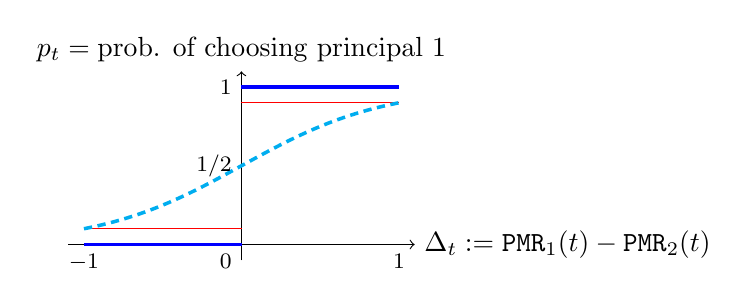
\begin{tikzpicture}[scale=2.0]
    \draw[->] (-1.1,0) -- (1.1,0) node[right] {$\Delta_t := \PMR_1(t) - \PMR_2(t)$};
    \draw[->] (0,-0.1) -- (0,1.1) node[above]
        {$p_t = \text{prob. of choosing principal 1}$};
    \draw[scale=1.0,domain=-1:0,smooth,variable=\q,blue, line width=0.50mm] plot ({\q},{0});
    \draw[scale=1.0,domain=0:1,smooth,variable=\q,blue,line width=0.50mm] plot ({\q},{1});
    \draw[scale=1.0,domain=-1:0,smooth,variable=\y,red]  plot ({\y},{0.1});
    \draw[scale=1.0,domain=0:1,smooth,variable=\y,red]  plot ({\y},{0.9});
    \draw[scale=1.0,domain=-1:1,smooth,variable=\y,cyan, line width=0.45mm, dash pattern=on 3pt off 2pt]  plot ({\y},{1/(1 + 1/(9^\y))});
    % \node[above, blue] at (0.5, 0.5) {\footnotesize $2 q (1 - q)$};
     \node[left] at (0, 0.5) {\footnotesize $1/2$};
     \node[left] at (0, 1) {\footnotesize $1$};
     \node[below left] at (0, 0) {\footnotesize $0$};
     \node[below ] at (1, 0) {\footnotesize $1$};
     \node[below ] at (-1, 0) {\footnotesize $-1$};
  \end{tikzpicture}
\end{center}
\caption{The three models for agents' response function: \HardMax is thick blue, \HardMaxRandom is slim red, and \SoftMaxRandom is the dashed curve.}
\label{fig:response-functions}
\end{figure}

\begin{OneLiners}
\item \HardMax: $\respF$ equals $0$ on the interval $[-1,0)$ and $1$
  on the interval $(0,1]$. In other words, the agents will
  deterministically choose the principal with the higher posterior
  mean reward.

\item \HardMaxRandom:
    % $\respF$ equals $\eps$ on the interval $[-1,0)$ and $1-\eps'$ on the interval $(0,1]$, where $\eps,\eps'\in (0,\tfrac12)$ are some positive constants. In words, each agent is a \HardMax agent with probability $1-\eps-\eps'$, and with the remaining probability she makes a random choice.
    $\respF$ equals $\eps_0$ on the interval $[-1,0)$ and $1-\eps_0$ on the interval $(0,1]$, where $\eps_0\in (0,\tfrac12)$ are some positive constants. In words, each agent is a \HardMax agent with probability $1-2\eps_0$, and with the remaining probability she makes a random choice.


\item \SoftMaxRandom: $\respF(\cdot)$ lies in the interval $[\eps_0,1-\eps_0]$, $\eps_0>0$, and is ``smooth" around $0$ (in the sense defined precisely in Section~\ref{sec:soft}).
\end{OneLiners}
% \asedit{(We assume $\respF(-1)+\respF(1)=1$ in \HardMaxRandom and \SoftMaxRandom only to simplify notation.)}

We say that $\respF$ is \emph{symmetric} if $\respF(-x)+\respF(x)=1$
for any $x\in [0,1]$. This implies \emph{fair tie-breaking}:
$\respF(0)=\tfrac12$.% , and $\eps=\eps'$ in the
% definitions above.

\xhdr{MAB algorithms.}
We characterize the inherent quality of an MAB algorithm in terms of its \emph{Bayesian Instantaneous Regret} (henceforth, \BIR), a standard notion from machine learning:
\begin{align}
\BIR(n) := \E_{\mu\sim\priorMu}
    \left[ \max_{a\in A} \mu_a\right] - \rew(n),
\end{align}
where $\rew(n)$ is the Bayesian-expected reward of the algorithm for the $n$-th step, when the algorithm is run in isolation. We are primarily interested in how \BIR scales with $n$; we treat $K$, the number of arms, as a constant unless specified otherwise.

We will emphasize several specific algorithms or classes thereof:

\begin{itemize}
\item ``smart" MAB algorithms that combine exploration and exploitation, such as UCB1 \cite{bandits-ucb1} and \gaedit{Thompson Sampling \cite{russo2018tutorial}}. These algorithms achieve
        $\BIR(n) \leq  \tilde{O}(n^{-1/2})$
    for all priors and all (or all but a very few) steps $n$. This bound is known to be tight for any fixed $n$.
    \footnote{This follows from the lower-bound analysis in \cite{bandits-exp3}.}

\item ``naive" MAB algorithms that separate exploration and exploitation, such as Explore-then-Exploit and $\eps$-Greedy. These algorithms have dedicated rounds in which they explore by choosing an action uniformly at random. When these rounds are known in advance, the algorithm suffers constant \BIR in such rounds. When the ``exploration rounds" are instead randomly chosen by the algorithm, one can usually guarantee an inverse-polynomial upper bound \BIR, but not as good as the one above: namely,
        $ \BIR(n) \leq \tilde{O}(n^{-1/3})$.
    This is the best possible upper bound on \BIR for the two algorithms mentioned above.

\item \DynGreedy: at each step, recommends the best action according to the current posterior: an action $a$ with the highest posterior expected reward
        $\E[\mu_a \mid \mI]$,
     where $\mI$ is the information available to the algorithm so far.
     \DynGreedy has (at least) a constant \BIR for some reasonable priors, \ie
        $\BIR(n)>\Omega(1)$.

\item \StaticGreedy: always recommends the prior best action,\ie an action $a$ with the highest prior mean reward  $\E_{\mu\sim \priorMu}[\mu_a]$. This algorithm typically has constant \BIR.
\end{itemize}

When we consider the analytical model, we focus on MAB algorithms such that $\BIR(n)$ is non-increasing; we call such algorithms \emph{monotone}. While some reasonable MAB algorithms may occasionally violate monotonicity, they can usually be easily modified so that monotonicity violations either vanish altogether, or only occur at very specific rounds (so that agents are extremely unlikely to exploit them in practice).

More background and examples can be found in Appendix~\ref{app:examples}. In particular, we prove that \DynGreedy is monotone.

\xhdr{Competition game between principals.}
Some of our results explicitly study the game between the two principals. We model it as a simultaneous-move game: before the first agent arrives, each principal commits to an MAB algorithm. Thus, choosing a pure strategy in this game corresponds to choosing an MAB algorithm (and, implicitly, announcing this algorithm to the agents).

Principal's utility is primarily defined as the market share, \ie the number of agents that chose this principal. Principals are risk-neutral, in the sense that they optimize their expected utility.

\xhdr{Assumptions on the prior.} We make some technical assumptions for the sake of simplicity. First, each action $a$ has a positive probability of being the best action according to the prior:
\begin{align}\label{eq:assn-prob}
\forall a\in A:\;\;\;  \Pr_{\mu\sim \priorMu}[\mu_a  > \mu_{a'}
\;\forall a'\in A]
> 0.
\end{align}

Second, posterior mean rewards of actions are pairwise distinct almost
surely. That is, the history $h$ at any step of an MAB algorithm%
\footnote{The \emph{history} of an MAB algorithm at a given step
  comprises the chosen actions and the observed rewards in all
  previous steps in the execution of this algorithm.}
 satisfies
\begin{align}\label{eq:assn-distinct}
    \E[\mu_a \mid h] \neq \E[\mu_{a'}\mid h] \quad \forall a,a'\in A,
\end{align}
\asedit{except at a set of histories of probability $0$}.  In
particular, prior mean rewards of actions are pairwise distinct:
$\E[\mu_a] \neq \E[\mu_a']$ for any $a,a'\in A$. 

We provide two examples for which property \eqref{eq:assn-distinct} is `generic', in the sense that it can be enforced almost surely by a
  small random perturbation of the prior. Both examples focus on 0-1 rewards and priors $\priorMu$ that are independent across arms. The first example
  assumes Beta priors on the mean rewards, and is very easy.%
  \footnote{Suppose the rewards are Bernouli r.v. and the mean reward
    $\mu_a$ for each arm $a$ is drawn from some Beta distribution
    $\text{Beta}(\alpha_a, \beta_a)$. Given any history that contains
    $h_a$ number of heads and $t_a$ number of tails from arm $a$, the
    posterior mean reward is
    $\frac{\alpha_a + h_a}{\alpha_a + h_a + \beta_a + t_a}$. Note that
    $h_a$ and $t_a$ take integer values. Therefore, perturbing the
    parameters $\alpha_a$ and $\beta_a$ independently with any
    continuous noise will induce a prior with property
    \eqref{eq:assn-distinct} with probability 1.  }  The second
  example assumes that mean rewards have a
  finite support, see Appendix~\ref{app:perturb} for details.

\xhdr{Some more notation.} Without loss of generality, we label actions as $A=[K]$ and sort them according to their prior mean rewards, so that
    $ \E[\mu_1] > \E[\mu_2] > \ldots > \E[\mu_K]$.

Fix principal $i\in \{1,2\}$ and (local) step $n$. The arm chosen by algorithm \alg[i] at this step is denoted $a_{i,n}$, and the corresponding \BIR is denoted $\BIR_i(n)$. History of \alg[i] up to this step is denoted $H_{i,n}$.
%The posterior distribution of agent $t$ for quantity $n_t(t)$ is denoted $\posteriorN{i}{t}$.

Write
    $\PMR(a\mid E) = \E[\mu_a \mid E]$
for posterior mean reward of action $a$ given event $E$.

%\end{assumption}

\subsection{Generalizations}
\label{sec:model-extensions}

Our results can be extended compared to the basic model described above.

%First, the two principals may have different action sets, as long as
%    $\E\left[ \max_{a\in A} \mu_a\right]$,
%the Bayesian-expected reward of the best action, is the same for both principals.

First, unless specified otherwise, our results allow a more general notion of principal's utility that can depend on both the market share and agents' rewards. Namely, principal $i$ collects $U_i(r_t)$ units of utility in each global round $t$ when she is chosen (and $0$ otherwise), where $U_i(\cdot)$ is some fixed non-decreasing function with $U_i(0)>0$. In a formula,
\begin{align}\label{eq:general-utility}
\textstyle U_i := \sum_{t=1}^T\; \indicator{i_t=i}\cdot U_i(r_r).
\end{align}

Second, our results carry over, with little or no modification of the proofs, to much more general versions of MAB, as long as it satisfies the i.i.d. property. In each round, an algorithm can see a \emph{context} before choosing an action (as in \emph{contextual bandits}) and/or additional feedback other than the reward after the reward is chosen (as in, \eg \emph{semi-bandits}), as long as the contexts are drawn from a fixed distribution, and the (reward, feedback) pair is drawn from a fixed distribution that depends only on the context and the chosen action. The Bayesian prior $\prior$ needs to be a more complicated object, to make sure that \PMR and \BIR are well-defined. Mean rewards may also have a known structure, such as Lipschitzness, convexity, or linearity; such structure can be incorporated via $\prior$. All these extensions have been studied extensively in the literature on MAB, and account for a substantial segment thereof; see \cite{Bubeck-survey12} for background and details.

\subsection{Chernoff Bounds}

We use an elementary concentration inequality known as {\em Chernoff Bounds}, in a formulation from~\cite{MitzUpfal-book05}.
\begin{theorem}[Chernoff Bounds]
\label{thm:chernoff}
Consider $n$ i.i.d. random variables $X_1 \ldots X_n$ with values in $[0,1]$. Let
    $X = \tfrac{1}{n} \sum_{i=1}^n X_i$ be their average, and let $\nu = \E[X]$. Then:
\[ \min\left(\; \Pr[ X-\nu > \delta \nu ],\quad
                \Pr[ \nu-X > \delta \nu ]
    \; \right)
    < e^{-\nu n \delta^2/3}
    \quad \text{for any $\delta\in (0,1)$.}
\]
\end{theorem}




%, and the choice of algorithm are commonly known
%to the agents. Given any finite class of MAB learning algorithms
%$\Pi$, a pure strategy for the principal $j$ in the competition game
%is an algorithm $\pi_j$ in the class $\Pi$ and a mixed strategy
%$\sigma_j$ is a probability distribution over $\Pi$. We will write
%$u_j(\sigma)$ and $u(\pi)$ to denote the expected utility for the
%principal $j$ in mixed strategy profile $\sigma$ and pure strategy
%profile $\pi$.  The principal gets a unit reward for being selected by
%an agent, so the utility function can be written as
%\[
%u_j(\pi) = \Ex{}{\sum_{t=1}^T\mathbf{1}[P^t = j]}
%\]
%A variant of the utility function we have is the number of agents
%weighted by the rewards for the agents
%\[
%u_j(\pi) = \Ex{}{\sum_{t=1}^T \mathbf{1}[P^t = j] r^t}
%\]
%\iffalse
%We consider a few models for the utility of the principals.  For
%example, the principal gets the reward realized by the agents it
%advised.
%\fi
%
%We will analyze the equilibrium strategies of the game under different
%environments.
%
%\begin{definition}[Equilibrium in the competition game]
%  A pure strategy profile $\pi$ is a pure strategy Nash equilibrium (PSNE) if
%  for any principal $j$ in the game and any algorithm $a\in \Pi$
%\[
%  u_j(\pi) \geq u_j(a, \pi_{-j}).
%\]
%A mixed strategy profile $\sigma$ is a (mixed strategy) Nash
%equilibrium if for any principal $j$ and any algorithm $a\in\Pi$,
%\[
%  \Ex{\sigma}{u_j(\sigma)} \geq u_j(a, \sigma_{-j}).
%\]
%\end{definition}
%
%We will measure the quality of an equilibrium by studying the welfare
%of the agents with respect to the system regret.



%%% Local Variables:
%%% TeX-master: "main.tex"
%%% End: 

\section{Full rationality (HardMax)}
\label{sec:rational}

In this section, we will consider the version in which
the agents are fully rational, in the sense that their response function is \HardMax. We show that principals are not incentivized to \emph{explore}--- \ie to deviate from \DynGreedy. The core technical result is that if one principal adopts \DynGreedy, then the other principal loses all agents as soon as he deviates.

To make this more precise, let us say that two MAB algorithms \emph{deviate} at (local) step $n$ if there is an action $a\in A$ and \asedit{a set of step-$n$ histories of positive probability such that any history $h$ in this set} is feasible for both algorithms, and under this history the two algorithms choose action $a$ with different probability.

\iffalse
\begin{definition}
  Suppose that an algorithm $\pi$ is not dynamic greedy. Then
  {\em the first exploration} for $\pi$ is the first time step where
  there is a non-zero probability that the recommended action has a
  lower expectation than exploitation option.\sw{define...}
\end{definition}
\fi


\begin{theorem}\label{thm:DG-dominance}
Assume \HardMax response function with fair tie-breaking. Assume that \alg[1] is \DynGreedy, and \alg[2] deviates from \DynGreedy starting from some (local) step $n_0<T$. Then all agents in global rounds $t\geq n_0$ select principal $1$.
\end{theorem}

\begin{corollary}\label{cor:DG-dominance}
The competition game between principals has a unique Nash equilibirium: both principals choose \DynGreedy.
\end{corollary}


\begin{remark}
This corollary holds under a more general model which allows time-discounting: namely, the utility of each principal $i$ in each global round $t$ is $U_{i,t}(r_t)$ if this principal is chosen, and $0$ otherwise, where $U_{i,t}(\cdot)$ is an arbitrary non-decreasing function with $U_{i,t}(0)>0$.
\end{remark}

\subsection{Proof of Theorem~\ref{thm:DG-dominance}}

The proof starts with two auxiliary lemmas: that deviating from \DynGreedy implies a strictly smaller Bayesian-expected reward, and that \HardMax implies a ``sudden-death" property: if one agent chooses principal $1$ with certainty, then so do all subsequent agents do. \asedit{We re-use both lemmas in later sections, so we state them in sufficient generality.}


\begin{lemma}\label{lm:DG-rew}
\asedit{Assume that \alg[1] is \DynGreedy, and \alg[2] deviates from \DynGreedy starting from some (local) step $n_0<T$. Then $\rew_1(n_0)>\rew_2(n_0)$. This holds for any response function $\respF$.}
\end{lemma}

\asedit{Lemma~\ref{lm:DG-rew} does not rely on any particular shape of the response function because it only considers the performance of each algorithm without competition.}

\begin{proof}[Proof of Lemma~\ref{lm:DG-rew}]
Since the two algorithms coincide on the first $n_0-1$ steps, it follows by symmetry that histories $H_{1,n_0}$ and $H_{2,n_0}$ have the same distribution. We use a \emph{coupling argument}: w.l.o.g., we assume the two histories coincide,
    $H_{1,n_0} = H_{2,n_0} = H$.

At local step $n_0$, \DynGreedy chooses an action $a_{1,n_0} = a_{1,n_0}(H)$
which maximizes the posterior mean reward given history $H$: for any realized history $h\in \support(H)$ and any action $a\in A$
\begin{align}\label{eq:lm:DG-rew-1}
 \PMR(a_{1,n_0} \mid H = h) \geq \PMR(a \mid H=h).
\end{align}

\ascomment{Rewrote the rest of the proof to account for positive-prob set of histories.}

By assumption \eqref{eq:assn-distinct}, it follows that 
\begin{align}\label{eq:lm:DG-rew-2}
 \PMR(a_{1,n_0} \mid H = h) > \PMR(a \mid H=h)
 \quad \text{for any $h\in \support(H)$ and $a\neq a_{1,n_0}(h)$.}
\end{align}

Since the two algorithms deviate at step $n_0$, there is a set $S\subset \support(H)$ of step-$n_0$ histories such that $\Pr[S]>0$ and any history $h\in S$ satisfies
    $\Pr[a_{2,n_0}\neq a_{1,n_0} \mid H=h]>0$.
Combining this with \eqref{eq:lm:DG-rew-2}, we deduce that 
\begin{align}\label{eq:lm:DG-rew-3}
 \PMR(a_{1,n_0} \mid H = h) > \E\left[ \mu_{a_{2,n_0}}\mid H=h \right]
 \quad\text{for each history $h\in S$}.
\end{align}
Using \eqref{eq:lm:DG-rew-1} and \eqref{eq:lm:DG-rew-3} and integrating over realized histories $h$, we obtain
    $\rew_1(n_0) > \rew_2(n_0)$.
\end{proof}


\begin{lemma}\label{lm:DG-sudden}
\asedit{Consider \HardMax response function with $\respF(0)\geq\tfrac12$.} 
Suppose \alg[1] is monotone, and $\PMR_1(t_0)>\PMR_2(t_0)$ for some global round $t_0$. Then $\PMR_1(t)>\PMR_2(t)$ for all subsequent rounds $t$.
\end{lemma}

\begin{proof}
Let us use induction on round $t\geq t_0$, with the base case $t=t_0$. Let $\mN=\mN_{1,t_0}$ be the agents' posterior distribution for $n_{1,t_0}$, the number of global rounds before $t_0$ in which principal $1$ is chosen. By induction, all agents from $t_0$ to $t-1$ chose principal $1$, so $\PMR_2(t_0)= \PMR_2(t)$. Therefore,
\[ \PMR_1(t)
    = \Ex{n\sim \mN}{\rew_1(n+1+t-t_0)}
    \geq \Ex{n\sim \mN}{\rew_1(n+1)}
    =\PMR_1(t_0) > \PMR_2(t_0)= \PMR_2(t), \]
where the first inequality holds because \alg[1] is monotone, and the second one is the base case.
\end{proof}

\begin{proof}[Proof of Theorem~\ref{thm:DG-dominance}]
Since the two algorithms coincide on the first $n_0-1$ steps, it follows by symmetry that $\rew_1(n) = \rew_2(n)$ for any $n< n_0$.
By Lemma~\ref{lm:DG-rew},
    $\rew_1(n_0) > \rew_2(n_0)$.

Recall that $n_i(t)$ is the number of global rounds $s<t$ in which principal $i$ is chosen, and $\posteriorN{i}{t}$ is the agents' posterior distribution for this quantity. By symmetry, each agent $t<n_0$ chooses a principal uniformly at random. It follows that
    $\posteriorN{1}{n_0} = \posteriorN{2}{n_0}$
(denote both distributions by $\mN$ for brevity), and $\mN(n_0-1)>0$.
Therefore:
\begin{align}
\PMR_1(n_0)
  &= \Ex{n\sim \mN} {\rew_1(n+ 1)}
   = \sum_{n = 0}^{n_0-1} \mN(n) \cdot{\rew_1(n + 1)} \nonumber \\
  & > \mN(n_0-1)\cdot {\rew_2(n_0)} + \sum_{n = 0}^{n_0-2}  \mN(n)\cdot{\rew_2(n + 1)}
    \nonumber \\
  &= \Ex{n\sim \mN}{\rew_2(n + 1)} = \PMR_2(n_0) \label{eq:pf:thm:DG-dominance}
\end{align}
So, agent $n_0$ chooses principal $1$. By Lemma~\ref{lm:DG-sudden} \asedit{(noting that \DynGreedy is monotone)}, all subsequent agents choose principal $1$, too.
\end{proof}


%\begin{theorem}
%  Suppose that the agents break ties uniformly at random, that is
%  $q=1/2$, then both principals playing \DynGreedy is the unique
%  equilibrium.
%\end{theorem}
%
%\begin{proof}
%  Suppose that both principals play dynamic greedy. The result
%  of Theorem~\ref{thm:DG-dominance} shows that there is no beneficial deviation
%  for both principals, so this forms a pure strategy equilibrium.
%
%  Now we will show that no other strategy profile can form equilibrium
%  in this game.  Suppose that both principals play some mixed
%  strategies that places non-zero probability on algorithms other than
%  dynamic greedy. We know one of the principals $p_j$ is getting no
%  more than $T/2$ agents in expectation. If $p_j$ switch to playing
%  only dynamic greedy, he can get strictly more than $T/2$ agents
%  by Theorem~\ref{thm:DG-dominance}. Thus, such a strategy profile will not form
%  an equilibrium.  Finally, suppose that $p_1$ plays dynamic greedy
%  and $p_2$ plays algorithms other than dynamic greedy with non-zero
%  probability. By Theorem~\ref{thm:DG-dominance}, we know that $p_2$ gets less
%  than $T/2$ agents in expectation. This means switching to dynamic
%  greedy will strictly improve the expected utility to $T/2$, so such
%  strategy profile cannot form an equilibrium either.
%\end{proof}


\subsection{\HardMax with biased tie-breaking}
\label{sec:HardMax-biased}

The \HardMax model is very sensitive to the tie-breaking rule. For starters, if ties are  broken deterministically in favor of principal $1$, then principal 1 can get all agents no matter what the other principal does, simply by using \StaticGreedy.

\begin{theorem}\label{thm:HardMax-hardTies}
Assume \HardMax response function with $\respF(0)=1$ (ties are always broken in favor of principal $1$). If \alg[1] is \StaticGreedy, then all agents choose principal $1$.
\end{theorem}

\begin{proof}
Agent $1$ chooses principal $1$ because of the tie-breaking rule. Since \StaticGreedy is trivially monotone, all the subsequent agents choose principal $1$ by an induction argument similar to the one in the proof of Lemma~\ref{lm:DG-sudden}.
\end{proof}

A more challenging scenario is when the tie-breaking is biased in favor of principal 1, but not deterministically so: $\respF(0)>\tfrac12$. Then this principal also has a ``winning strategy" no matter what the other principal does. Specifically, principal 1 can get all but the first few agents, under a mild technical assumption that \DynGreedy deviates from \StaticGreedy. Principal 1 can use \DynGreedy, or any other monotone MAB algorithm that coincides with \DynGreedy in the first few steps.

%We can generalize the theorem top the case of $q >1/2$ if the
%principal $p_1$ can guarantee better than the a priori best action to
%all the agents following the second.


\begin{theorem}\label{thm:HardMax-biased}
Assume \HardMax response function with $\respF(0)>\tfrac12$ (\ie tie-breaking is biased in favor of principal $1$). Assume the prior $\mP$ is such that \DynGreedy deviates from \StaticGreedy starting from some step $n_0$. Suppose that principal $1$ runs a monotone MAB algorithm that coincides with \DynGreedy in the first $n_0$ steps. Then all agents $t\geq n_0$ choose principal $1$.
\end{theorem}


\begin{proof}
The proof re-uses Lemmas~\ref{lm:DG-rew} and~\ref{lm:DG-sudden}, which do not rely on fair tie-breaking.

Because of the biased tie-breaking, for each global round $t$ we have:
\begin{align}\label{eq:thm:HardMax-biased-PMRtoPr}
\text{if $\PMR_1(t)\geq \PMR_2(t)$ then $\Pr[i_t=1]>\tfrac12$.}
\end{align}
Recall that $i_t$ is the principal chosen in global round $t$.

Let $m_0$ be the first step when \alg[2] deviates from \DynGreedy, or \DynGreedy deviates from \StaticGreedy, whichever comes sooner. \asedit{Then \alg[2], \DynGreedy and \StaticGreedy coincide on the first $m_0-1$ steps. Moreover, $m_0\leq n_0$ (since \DynGreedy deviates from \StaticGreedy at step $n_0$), so \alg[1] coincides with \DynGreedy on the first $m_0$ steps.

So, $\rew_1(n)=\rew_2(n)$ for each step $n<m_0$, because \alg[1] and \alg[2] coincide on the first $m_0-1$ steps. Moreover, if \alg[2] deviates from \DynGreedy at step $m_0$ then
    $\rew_1(m_0) > \rew_2(m_0)$ 
by Lemma~\ref{lm:DG-rew}; else, we trivially have
    $\rew_1(m_0) = \rew_2(m_0)$.} To summarize:
\begin{align}\label{eq:thm:HardMax-biased-rew}
    \rew_1(n)\geq\rew_2(n)\quad \text{for all steps $n\leq m_0$}.
\end{align}

We claim that $\Pr[i_t=1]>\tfrac12$ for all global rounds $t\leq m_0$. We prove this claim using induction on $t$. The base case $t=1$ holds by \eqref{eq:thm:HardMax-biased-PMRtoPr} and the fact that in step 1, \DynGreedy chooses the arm with the highest prior mean reward. For the induction step, we assume that $\Pr[i_t=1]>\tfrac12$ for all global rounds $t<t_0$, for some $t_0\leq  m_0$. It follows that distribution $\posteriorN{1}{t_0}$ stochastically dominates distribution $\posteriorN{2}{t_0}$.%
\footnote{For random variables $X,Y$ on \R, we say that $X$ \emph{stochastically dominates} $Y$ if $\Pr[X\geq x] \geq \Pr[Y\geq x]$ for any $x\in \R$.}
Observe that
\begin{align}\label{eq:thm:HardMax-biased-PMR-aux}
\PMR_1(t_0)
  = \Ex{n\sim \posteriorN{1}{t_0}} {\rew_1(n+1)}
  \geq \Ex{n\sim \posteriorN{2}{t_0}} {\rew_2(n+1)}
  = \PMR_2(t_0).
\end{align}
So the induction step follows by \eqref{eq:thm:HardMax-biased-PMRtoPr}. Claim proved.

Now let us focus on global round $m_0$, and denote $\mN_i = \posteriorN{i}{m_0}$.  By the above claim,
\begin{align}\label{eq:thm:HardMax-biased-mN}
\text{$\mN_1$ stochastically dominates $\mN_2$, and moreover
    $\mN_i(m_0-1)>\mN_i(m_0-1)$.}
\end{align}

By definition of $m_0$, either (i) \alg[2] deviates from \DynGreedy starting from local step $m_0$, which implies $\rew_1(m_0)> \rew_2(m_0)$ by Lemma~\ref{lm:DG-rew}, or (ii) \DynGreedy deviates from \StaticGreedy starting from local step $m_0$, which implies $\rew_1(m_0)>\rew_1(m_0-1)$ by Lemma~\ref{dgmono}. In both cases, using \eqref{eq:thm:HardMax-biased-rew} and \eqref{eq:thm:HardMax-biased-mN}, it follows that the inequality in \eqref{eq:thm:HardMax-biased-PMR-aux} is strict for $t_0=m_0$.

Therefore, agent $m_0$ chooses principal $1$, and by Lemma~\ref{lm:DG-sudden} so do all subsequent agents.
\end{proof}


% OLD PROOF (assuming alg1 coincides with DG on first two rounds, etc.
% We consider two cases, depending on the arm $a_{2,1}$ that principal $2$ chooses in the same step. The interesting case is $a_{2,1}=1$.
%Then agent $1$ selects principal $1$ with probability $q:=\respF(0)>\tfrac12$. Therefore, agent $2$ forms the following posterior mean rewards:
%\begin{align*}
%  \PMR_1(2) &= (1-q)\cdot \E[\mu_1] + q\cdot \rew_1(2)
%    \EqComment{for principal 1}\\
%  \PMR_2(2) &= q\cdot \E[\mu_1] + (1-q)\cdot \rew_2(2)
%    \EqComment{for principal 2}.
%\end{align*}
%We know that
%    $\rew_1(2) > \E[\mu_1]$
%(\DynGreedy is strictly monotone in the first $2$ rounds)
%from Lemma~\ref{dgmono}, and
%    $\rew_1(2) \geq \rew_2(2)$
%by Lemma~\ref{lm:DG-rew}. It follows that
%    $\PMR_1(2)>\PMR_2(2)$,
%and consequently agent $2$ chooses principal $1$. The subsequent agents choose principal $1$ by Lemma~\ref{lm:DG-sudden}.
%
%The remaining case is $a_{2,1}\neq 1$: principal $p_2$ does not recommend arm $1$ in the first step. Since all other arms have a strictly lower prior mean reward, agent $1$ chooses principal $1$. The subsequent agents choose principal $1$ by Lemma~\ref{lm:DG-sudden}.



% \begin{lemma}
%   Let $\mu^2_{DG}$ the expected reward of action of \DynGreedy
%   in the second step. Then $\mu^2_{DG} > \mu_1$.
% \end{lemma}

% \begin{proof}
%   \sw{todo. This requires an assumption that the second arm has
%     non-zero probability of beating the first one.}
% \end{proof}



% Steven's proof for a more general version with alg1 = BIC algo
%Agent $1$ chooses principal $1$ because of the tie-breaking rule,
%  Since principal $p_1$ in the first step recommends arm 1, the agent
%  selects principal $p_1$ (due to the tie breaking rule).  Agent $2$
%  knows that agent $1$ selected $p_1$. Because of BIC, she knows $p_1$
%  will offer reward no lower than $p_2$ in expectation.  By induction,
%  all the agents select principal $p_1$.



%\sw{We also have an observation saying if one principal starts with a
%  better dynamic greedy will just dominate the game. It could do some
%  amount of exploration while having better Bayesian per-round regret
%  than the other principal. This means the other principal will never
%  have any agents arriving for learning.}

%%% Local Variables:
%%% TeX-master: "main.tex"
%%% End: 

\section{Relaxed rationality: HardMax \& Random}
\label{sec:random}
This section is dedicated to the \HardMaxRandom response model, where each principal is always chosen with some positive baseline probability. The main technical result for this model states that a principal with asymptotically better \BIR wins by a large margin: after a ``learning phase" of constant duration, all agents choose this principal with maximal possible probability $\respF(1)$. For example, a principal with $\BIR(n)\leq \tilde{O}(n^{-1/2})$ wins over a principal with $\BIR(n)\geq \Omega(n^{-1/3})$. However, this positive result comes with a significant caveat detailed in Section~\ref{sec:random-greedy}.

We formulate and prove a cleaner version of the result, followed by a more general formulation developed in a subsequent Remark~\ref{rem:random-messy}. We need to express a property that \alg[1] eventually catches up and surpasses \alg[2], even if initially it receives only a fraction of traffic. For the cleaner version, we assume that both algorithms are well-defined for an infinite time horizon, so that their \BIR does not depend on the time horizon $T$ of the game.  Then this property can be formalized as:
\begin{align}\label{eq:random-better-clean}
(\forall \eps>0)\qquad
\BIR_1(\eps n)/\BIR_2(n) \to 0.
\end{align}
In fact, a weaker version of \eqref{eq:random-better-clean} suffices:
denoting $\eps_0 = \respF(-1)$, for some constant $n_0$ we have
\begin{align}\label{eq:random-better-weaker}
(\forall n\geq n_0) \qquad
\BIR_1(\eps_0 n/2)/\BIR_2(n) <\tfrac12.
\end{align}
We also need a very mild technical assumption on the ``bad" algorithm:
\begin{align}\label{eq:random-assn}
 (\forall n\geq n_0) \qquad
  \BIR_2(n) > 4\,e^{-\eps_0 n/12}.
\end{align}

\begin{theorem}\label{thm:random-clean}
Assume \HardMaxRandom response function. Suppose both algorithms are monotone and well-defined for an infinite time horizon, and satisfy~\eqref{eq:random-better-weaker} and~\eqref{eq:random-assn}. Then each agent $t\geq n_0$ chooses principal $1$ with maximal possible probability $\respF(1) = 1- \eps_0$.
\end{theorem}

\begin{proof}
Consider global round $t\geq n_0$. Recall that each agent chooses principal $1$ with probability at least
    $\respF(-1)>0$.

Then
    $\E[n_1(t+1)] \geq 2\eps_0\,t $.
By Chernoff Bounds (Theorem~\ref{thm:chernoff}), we have that
    $n_1(t+1)\geq \eps_0 t$
holds with probability at least $1-q$,
where $q = \exp(-\eps_0 t/12)$.

We need to prove that
    $\PMR_1(t) - \PMR_2(t)>0$.
For any $m_1$ and $m_2$, consider the quantity
\[ \Delta(m_1,m_2) := \BIR_2(m_2+1) - \BIR_1(m_1+1).\]
Whenever $m_1 \geq \eps_0 t/2 -1$ and $m_2<t$, it holds that
\begin{align*}
\Delta(m_1,m_2) \geq \Delta(\eps_0 t / 2, t)
    \geq \BIR_2(t)/2.
\end{align*}
The above inequalities follow, resp., from algorithms' monotonicity and \eqref{eq:random-better-weaker}. Now,
\begin{align*}
\PMR_1(t) - \PMR_2(t)
    &= \Ex{m_1\sim \posteriorN{1}{t},\;m_2\sim \posteriorN{2}{t}}{\Delta(m_1,m_2)} \\
    &\geq -q
        + \Ex{m_1\sim \posteriorN{1}{t},\;m_2\sim \posteriorN{2}{t}}
            {\Delta(m_1,m_2)\mid m_1 \geq \eps_0 t/2-1} \\
    &\geq \BIR_2(t)/2-q \\
    &> \BIR_2(t)/4 > 0  \EqComment{by \eqref{eq:random-assn}}. \qedhere
\end{align*}
\end{proof}

\begin{remark}\label{rem:random-messy}
  Many standard MAB algorithms in the literature are parameterized by
  the time horizon $T$. Regret bounds for such algorithms usually
  include a polylogarithmic dependence on $T$. In particular, a
  typical upper bound for \BIR has the following form:
  \OMIT{\footnote{We
    provide upper bounds on \BIR for several standard MAB algorithms
    to illustrate these dependencies in the appendix.\sw{added}}}
\begin{align}
    \BIR(n\mid T)\leq \polylog(T)\cdot n^{-\gamma}
    \quad \text{for some $\gamma\in(0,\tfrac12]$}.
\end{align}
Here we write $\BIR(n\mid T)$ to emphasize the dependence on $T$.

We generalize \eqref{eq:random-better-weaker} to handle the dependence
on $T$: there exists a number $T_0$ and a function $n_0(T)\in \polylog(T)$ 
such that 
\begin{align}\label{eq:random-better-messy}
(\forall T\geq T_0,\; n\geq n_0(T)) \quad
\frac{\BIR_1(\eps_0 n /2\mid T)}{\BIR_2(n\mid T)} <\frac12.
\end{align}
If this holds, we say that \alg[1] \emph{BIR-dominates} \alg[2].

We provide a version of Theorem~\ref{thm:random-clean} in which algorithms are parameterized with time horizon $T$ and condition \eqref{eq:random-better-weaker} is replaced with \eqref{eq:random-better-messy}; its proof is very similar and is omitted.
\end{remark}

%\begin{theorem}\label{thm:random-messy}
%Assume \HardMaxRandom response function, and algorithms that satisfy \eqref{eq:random-better-messy} and~\eqref{eq:random-assn}. Then each agent
%    $t\geq n_0(T)$ chooses principal $1$ with probability $\respF(1)$.
%\end{theorem}


%Let \alg be a monotone MAB algorithm and $\mA$ be a finite set of monotone MAB algorithms such that each algorithm in $\mA$ satisfies \eqref{eq:random-assn} and is ``dominated" by \alg in the sense of \eqref{eq:random-better-messy}.
%Assume principals can only choose algorithms from $\mA\cup \{\alg\}$.

To state a game-theoretic corollary of Theorem~\ref{thm:random-clean}, we consider a version of the competition game between the two principals in which they can only choose from a finite set $\mA$ of monotone MAB algorithms. One of these algorithms is ``better" than all others; we call it the \emph{special} algorithm. Unless specified otherwise, it BIR-dominates all other allowed algorithms. The other algorithms satisfy \eqref{eq:random-assn}. We call this game the \emph{restricted competition game}.

\begin{corollary}\label{cor:random}
Assume \HardMaxRandom response function. Consider the restricted competition game with special algorithm \alg. Then, for any sufficiently large time horizon $T$, this game has a unique Nash equilibrium: both principals choose \alg.
\end{corollary}


\subsection{A little greedy goes a long way}
\label{sec:random-greedy}

Given any monotone MAB algorithm other than \DynGreedy, we design a modified algorithm which learns at a slower rate, yet ``wins the game" in the sense of Theorem~\ref{thm:random-clean}. As a corollary, the competition game with unrestricted choice of algorithms typically does not have a Nash equilibrium.

Given an algorithm \alg[1] that deviates from \DynGreedy starting from
step $n_0$ and a ``mixing'' parameter $p$, we will construct a
modified algorithm as follows.
\begin{enumerate}
\item The modified algorithm coincides with \alg[1] (and \DynGreedy)
for the first $n_0-1$ steps;
\item In each step $n\geq n_0$, \alg[1] is invoked with probability
  $1-p$, and with the remaining probability $p$ does the ``greedy
  choice": chooses an action with the largest posterior mean reward
  given the current information collected by \alg[1].
\end{enumerate}
%The modified algorithm is called \emph{greedy deviation}, with probability parameter $p$.
For a cleaner comparison between the two algorithms, the modified algorithm does not record rewards received in steps with the ``greedy choice". Parameter $p>0$ is the same for all steps.

\begin{theorem}\label{thm:random-greedy}
Assume symmetric \HardMaxRandom response function. Let $\eps_0 = \respF(-1)$ be the baseline probability. Suppose \alg[1] deviates from \DynGreedy starting from some step $n_0$. Let \alg[2] be the modified algorithm, as described above, with mixing parameter $p$ such that
    $(1-\eps_0)(1-p)>\eps_0$.
Then each agent $t\geq n_0$ chooses principal $2$ with maximal possible probability $1-\eps_0$.
\end{theorem}

\begin{corollary}\label{cor:random-greedy}
  Suppose that both principals can choose any monotone MAB algorithm, and assume the symmetric \HardMaxRandom response
  function. Then for any time
  horizon $T$, the only possible \emph{pure} Nash equilibrium is one
  where both principals choose \DynGreedy. Moreover, no pure Nash
  equilibrium exists when some algorithm ``dominates" \DynGreedy in
  the sense of \eqref{eq:random-better-messy} and the time horizon $T$
  is sufficiently large.
\end{corollary}


\begin{remark}
The modified algorithm performs exploration % ingests information
at a slower rate. Let us argue how this may translate  into a larger \BIR compared to the original algorithm. Let  $\BIR'_1(n)$ be the \BIR of the ``greedy choice" after after $n-1$ steps of \alg[1]. Then
\begin{align}\label{eq:random-BIR}
\BIR_2(n)
    &= \Ex{m\sim (n_0-1)+\term{Binomial}(n-n_0+1,1-p)}{(1-p) \cdot \BIR_1(m) + p \cdot \BIR'_1(m)}.
\end{align}
In this expression, $m$ is the number of times \alg[1] is invoked in the first $n$ steps of the modified algorithm. Note that
    $\E[m] = n_0-1 + (n-n_0+1)(1-p) \geq (1-p)n$.

Suppose $\BIR_1(n)= \beta n^{-\gamma}$ for some constants $\beta,\gamma>0$. Further, assume 
    $\BIR'_1(n)\geq  c\; \BIR_1(n)$,
for some $c>1-\gamma$.
Then for all $n\geq n_0$ and small enough $p>0$ it holds that:
\begin{align*}
 \BIR_2(n) 
    &\geq  (1-p+pc)\; \E[\; \BIR_1(m) \;] \\
\E[\; \BIR_1(m) \;]
    &\geq \BIR_1(\; \E[m] \;) &\qquad\text{(By Jensen's inequality)} \\
    &\geq \BIR_1(\; (1-p)n \;) &\qquad\text{(since $\E[m]\geq n(1-p)$)}  \\
    &\geq \beta\cdot n^{-\gamma} \cdot (1-p)^{-\gamma} 
        &\qquad\text{(plugging in $\BIR_1(n)=\beta n^{-\gamma}$)}  \\
    &> \BIR_1(n)\;\; (1-p\gamma)^{-1}
        &\qquad\text{(since $(1-p)^\gamma < 1-p\gamma$)}.\\
\BIR_2(n) 
    &>\alpha\cdot \BIR_1(n),
    &\text{where} \quad 
    \alpha = \tfrac{1-p+pc}{1-p\gamma}>1.
\end{align*}
(In the above equations, all expectations are over $m$ distributed as in \eqref{eq:random-BIR}.)
\end{remark}


\begin{proof}[Proof of Theorem~\ref{thm:random-greedy}]
  Let $\rew'_1(n)$ denote the Bayesian-expected reward of the ``greedy
  choice'' after after $n-1$ steps of \alg[1]. Note that
  $\rew_1(\cdot)$ and $\rew'_1(\cdot)$ are non-decreasing: the former
  because \alg[1] is monotone and the latter because the ``greedy
  choice'' is only improved with an increasing set of
  observations. Therefore, the modified algorithm \alg[2] is monotone
  by \eqref{eq:random-BIR}.

  By definition of the ``greedy choice,'' $\rew_1(n)\leq \rew'_1(n)$
  for all steps $n$. Moreover, by Lemma~\ref{lm:DG-rew},
  \alg[1] has a strictly smaller $\rew(n_0)$ compared to \DynGreedy;
  so, $\rew_1(n_0)<\rew_2(n_0)$.

Let $\alg$ denote a copy of \alg[1] that is running ``inside" the modified algorithm \alg[2]. Let $m_2(t)$ be the number of global rounds before $t$ in which the agent chooses principal $2$ \emph{and} \alg is invoked; in other words, it is the number of agents seen by \alg before global round $t$. Let $\mM_{2,t}$ be the agents' posterior distribution for $m_2(t)$.

We claim that in each global round $t\geq n_0$, distribution $\mM_{2,t}$ stochastically dominates distribution $\posteriorN{1}{t}$, and $\PMR_1(t)<\PMR_2(t)$. We use induction on $t$. The base case $t=n_0$ holds because $\mM_{2,t} = \posteriorN{1}{t}$ (because the two algorithms coincide on the first $n_0-1$ steps), and $\PMR_1(n_0)<\PMR_2(n_0)$ is proved as in \eqref{eq:pf:thm:DG-dominance}, using the fact that $\rew_1(n_0)<\rew_2(n_0)$.

The induction step is proved as follows. The induction hypothesis for global round $t-1$ implies that agent $t-1$ is seen by \alg with probability $(1-\eps_0)(1-p)$, which is strictly larger than $\eps_0$, the probability with which this agent is seen by \alg[2]. Therefore, $\mM_{2,t}$ stochastically dominates $\posteriorN{1}{t}$.
\begin{align}
\PMR_1(t)
  &= \Ex{n\sim \posteriorN{1}{t}} {\rew_1(n+1)} \nonumber \\
  &\leq \Ex{m\sim \mM_{2,t}} {\rew_1(m+1)}
    \label{eq:pf:thm:random-greedy-1}\\
  &< \Ex{m\sim \mM_{2,t}} {(1-p)\cdot \rew_1(m+1) + p\cdot \rew'_1(m+1)}
    \label{eq:pf:thm:random-greedy-2} \\
  &= \PMR_2(t). \nonumber
\end{align}
Here inequality \eqref{eq:pf:thm:random-greedy-1} holds because $\rew_1(\cdot)$ is monotone and $\mM_{2,t}$ stochastically dominates $\posteriorN{1}{t}$, and inequality \eqref{eq:pf:thm:random-greedy-2} holds because $\rew_1(n_0)<\rew_2(n_0)$ and $\mM_{2,t}(n_0)>0$.%
\footnote{If $\rew_1(\cdot)$ is strictly increasing, then inequality \eqref{eq:pf:thm:random-greedy-1} is strict, too; this is because $\mM_{2,t}(t-1)>\posteriorN{1}{t}(t-1)$.  }
\end{proof}



%%% Local Variables:
%%% TeX-master: "main.tex"
%%% End: 

\section{SoftMax response function}
\label{sec:soft}
This section is devoted to the \SoftMaxRandom model. We recover a positive result under the assumptions from Theorem~\ref{thm:random-clean} (albeit with a weaker conclusion), and then proceed to a much more challenging result under weaker assumptions. We start with a formal definition:

\begin{definition}\label{def:SoftMax}
A response function $\respF$ is \SoftMaxRandom if the following conditions hold:
\begin{OneLiners}
\item  $\respF(\cdot)$ is bounded away from $0$ and $1$:
    $\respF(\cdot)\in [\eps,1-\eps]$ for some $\eps\in (0,\tfrac12)$,
\item  the response function
 $\respF(\cdot)$ is ``smooth" around $0$:
 \begin{align}\label{eq:SoftMax-smooth}
 \exists\, \text{constants $\delta_0,c_0,c'_0>0$}
    \qquad \forall x\in [-\delta_0,\delta_0] \qquad
    c_0 \leq \respF'(x) \leq c'_0.
 \end{align}
\item fair tie-breaking: $\respF(0)=\tfrac12$.
\end{OneLiners}
\end{definition}

\begin{remark}
\asedit{This definition is fruitful when parameters $c_0$ and $c_0'$ are close to $\tfrac12$. Throughout, we assume that \alg[1] is better than \alg[2], and obtain results parameterized by $c_0$. By symmetry, one could assume that \alg[2] is better than \alg[1], and obtain similar results parameterized by $c_0'$.}
\end{remark}

Our first result is a version of Theorem~\ref{thm:random-clean}, with the same assumptions about the algorithms and essentially the same proof. The conclusion is much weaker: we can only guarantee that each agent $t\geq n_0$ chooses principal 1 with probability slightly larger than $\tfrac12$. This is essentially unavoidable in a typical case when both algorithms satisfy $\BIR(n)\to 0$, by Definition~\ref{def:SoftMax}.

\begin{theorem}\label{thm:SoftMax-weak}
  Assume \SoftMaxRandom response function. Suppose \alg[1] has better
  \BIR in the sense of \eqref{eq:random-better-weaker}, and \alg[2]
  satisfies the condition \eqref{eq:random-assn}. Then each agent
  $t\geq n_0$ chooses principal $1$ with probability
\begin{align}\label{eq:thm:SoftMax-weak}
     \Pr[i_t = 1]\geq \tfrac12 +  \tfrac{c_0}{4}\; \BIR_2(t).
\end{align}
\end{theorem}

\begin{proof}[Proof Sketch]
We follow the steps in the proof of Theorem~\ref{thm:random-clean} to derive \begin{align*}
\PMR_1(t) - \PMR_2(t)
    &\geq \BIR_2(t)/2 -q,
    \quad \text{where $q = \exp(-\eps_0 t/12)$.}
\end{align*}
This is at least $\BIR_2(t)/4$ by \eqref{eq:random-assn}. Then \eqref{eq:thm:SoftMax-weak} follows by the smoothness condition \eqref{eq:SoftMax-smooth}.
\end{proof}

We recover a version of Corollary~\ref{cor:random}, if each principal's utility is the number of users (rather than the more general model in \eqref{eq:general-utility}). We also need a mild technical assumption that cumulative Bayesian regret (\BReg) tends to infinity. \BReg is a standard notion from the literature (along with \BIR):
\begin{align}\label{eq:SoftMax-BReg}
\BReg(n) := n\cdot \E_{\mu\sim\priorMu}
    \left[ \max_{a\in A} \mu_a\right] - \sum_{n=1}^n \rew(n')
    = \sum_{n'=1}^n \BIR(n').
\end{align}

\begin{corollary}\label{cor:SoftMax}
Assume that the response function is \SoftMaxRandom, and each principal's  utility is the number of users.
%
%Suppose principals can only choose algorithms from $\mA\cup \{\alg\}$, where $\mA\cup \{\alg\}$ is a finite set of monotone MAB algorithms such that each algorithm in $\mA$ satisfies \eqref{eq:random-assn} and $\BReg(n)\to \infty$, and is ``dominated" by \alg in the sense of \eqref{eq:random-better-messy}.
%
Consider the restricted competition game with special algorithm \alg, and assume that all other allowed algorithms satisfy $\BReg(n)\to \infty$. Then, for any sufficiently large time horizon $T$, this game has a unique Nash equilibrium: both principals choose \alg.
\end{corollary}

Further, we prove a much more challenging result in which the
condition \eqref{eq:random-better-weaker} is replaced with a much
weaker ``BIR-dominance'' condition. For clarity, we will again assume
that both algorithms are well-defined for an infinite time
horizon. The \emph{weak BIR dominance} condition says there exist
constants $\beta_0, \alpha_0\in (0, 1/2)$ and $n_0$ such that
 \begin{align}\label{eq:SoftMax-better}
   (\forall n\geq n_0) \quad
   \frac{\BIR_1((1-\beta_0)\, n)}{\BIR_2(n)} <1-\alpha_0.
 \end{align}
% for some $n_0(T)\in \polylog(T)$ and constants
% $\beta_0,\alpha_0\in (0, 1/2)$,
% \begin{align}\label{eq:SoftMax-better}
% (\forall n\geq n_0(T)) \quad
% \frac{\BIR_1((1-\beta_0)\, n\mid T)}{\BIR_2(n\mid T)} <1-\alpha_0.
% \end{align}
 If this holds, we say that \alg[1] \emph{weakly BIR-dominates}
 \alg[2]. Note that the condition \eqref{eq:random-better-messy}
 involves sufficiently small multiplicative factors (resp., $\eps_0/2$
 and $\tfrac12$), the new condition replaces them with factors that
 can be arbitrarily close to $1$.

 We make a mild assumption on \alg[1] that its $\BIR_1(n)$ tends to
 0. Formally, for any $\eps > 0$, there exists some $n(\eps)$ such
 that
 \begin{align}\label{eq:so-mild}
   (\forall n\geq n(\eps)) \qquad \BIR_1(n) \leq \eps.
 \end{align}
 We also require a slightly stronger version of the technical
 assumption~\eqref{eq:random-assn}:%  for any $\eps > 0$, there exists
 % $n(\eps)$ such that for
for some $n_0$,
\begin{align}\label{eq:SoftMax-assn-strong}
 % (\forall n\geq n(\eps)) \qquad
 %  \BIR_2(n) > e^{-\eps n}. %used to be 4exp( -\eps n/6)
(\forall n\geq n_0) \qquad 
\BIR_2(n) \geq \frac{4}{\alpha_0} \exp \left( \frac{-\min\{\eps_0, 1/8\} n}{12}\right)
\end{align}




\begin{theorem}\label{thm:SoftMax-strong}
  Assume the \SoftMaxRandom response function. Suppose \alg[1]
  weakly-BIR-dominates \alg[2], \alg[1] satisfies \eqref{eq:so-mild},
  and \alg[2] satisfies \eqref{eq:SoftMax-assn-strong}. Then there
  exists some $t_0$ such that each agent $t\geq t_0$ chooses principal
  $1$ with probability
\begin{align}\label{eq:thm:SoftMax-strong}
     \Pr[i_t = 1]\geq \tfrac12 +  \tfrac{c_0\alpha_0}{4}\; \BIR_2(t).
\end{align}
\end{theorem}




The main idea behind our proof is that even though \alg[1] may have a
slower rate of learning in the beginning, it will gradually catch up
and surpass \alg[2]. We will describe this process in two phases. In
the first phase, \alg[1] receives a random agent with probability at
least $\respF(-1) = \eps_0$ in each round. Since $\BIR_1$ tends to 0,
the difference in \BIR{s} between the two algorithms is also
diminishing. Due to the \SoftMaxRandom response function, \alg[1]
attracts each agent with probability at least $1/2 - O(\beta_0)$ after
a sufficient number of rounds. Then the game enters the second phase:
both algorithms receive agents at a rate close to $\tfrac12$, and the
fractions of agents received by both algorithms --- $n_1(t)/t$ and
$n_2(t)/t$ --- also converge to $\tfrac12$. At the end of the second
phase and in each global round afterwards, the counts $n_1(t)$ and
$n_2(t)$ satisfy the weak BIR-dominance condition, in the sense that
they both are larger than $n_0$ and $n_1(t)\geq (1-\beta_0)\; n_2(t)$.
At this point, \alg[1] actually has smaller $\BIR$, which reflected in the {\PMR}s eventually. Accordingly, from then on \alg[1]
attracts agents at a rate slightly larger than $\tfrac12$. We prove
that the ``bump'' over $\tfrac12$ is at least on the order of
$\BIR_2(t)$.


\begin{proof}[Proof of Theorem~\ref{thm:SoftMax-strong}]
  Let $\beta_1 = \min\{c_0'\delta_0, \beta_0/20\}$ with $\delta_0$
  defined in~\eqref{eq:SoftMax-smooth}.  Recall each agent chooses
  \alg[1] with probability at least $\respF(-1)= \eps_0$.  By
  condition \eqref{eq:so-mild} and \eqref{eq:SoftMax-assn-strong},
  there exists some sufficiently large $T_1$ such that for any
  $t\geq T_1$, $\BIR_1(\eps_0 T_1/2) \leq \beta_1/c_0'$ and
  $\BIR_2(t) > e^{-\eps_0 t/12}$. Moreover, for any $t\geq T_1$, we
  know $\E[n_1(t+1)] \geq \eps_0\,t $, and by the Chernoff Bounds
  (Theorem~\ref{thm:chernoff}), we have $n_1(t+1) \geq \eps_0 t/2$
  holds with probability at least $1 - q_1(t)$ with
  $q_1(t) = \exp(-\eps_0 t/12) < \BIR_2(t)$. It follows that for any $t\geq T_1$,
\begin{align*}
  \PMR_2(t) - \PMR_1(t) &= \Ex{m_1\sim \posteriorN{1}{t},\;m_2\sim \posteriorN{2}{t}}{\BIR_1(m_1+ 1) - \BIR_2(m_2+1)} \\
                        &\leq q_1(t)  + \Ex{m_1\sim \posteriorN{1}{t}}{\BIR_1(m_1+ 1)\mid m_1 \geq \eps_0 t/2 - 1 } - \BIR_2(t)\\
                        &\leq \BIR_1(\eps_0 T_1/2) \leq \beta_1/c_0'
\end{align*}
% where the second inequality follows from~\eqref{eq:random-assn}.
Since the response function $\respF$ is $c_0'$-Lipschitz in the
neighborhood of $[-\delta_0, \delta_0]$, each agent after round $T_1$
will choose \alg[1] with probability at least
\[
  p_t \geq \frac{1}{2} - c_0'\left(\PMR_2(t) - \PMR_1(t)\right) \geq
  \frac{1}{2} - \beta_1.
\]

Next, we will show that there exists a sufficiently large $T_2$ such
that for any $t\geq T_1 + T_2$, with high probability
$n_1(t) > \max\{n_0, (1 - \beta_0)n_2(t)\}$, where $n_0$ is defined
in~\eqref{eq:SoftMax-better}. %  Let us first lower bound the number of
% agents received by \alg[1] after some number of rounds $t = T_1 + T'$
% for any $T' \geq T_1$. 
Fix any $t \geq T_1 + T_2$. 
Since each agent chooses \alg[1] with probability at least
$1/2 - \beta_1$, by Chernoff Bounds (Theorem~\ref{thm:chernoff}) we
have with probability at least $1 - q_2(t)$ that the number of agents
that choose \alg[1] is at least $\beta_0(1/2 - \beta_1)t/5$, where the
function
$$
q_2(x) = \exp\left( \frac{-(1/2 - \beta_1)(1 - \beta_0/5)^2x}{3} \right).
$$
Note that the number of agents received by \alg[2] is at most
$T_1 + (1/2 + \beta_1)t + (1/2 - \beta_1)(1 - \beta_0/5)t$.

Then as long as
% $T_2 \geq \max\left\{\frac{3T_1}{(1 - \beta_0)}, 8 n_0\right\}$, we
% can guarantee that for any $t \geq T_1 + T_2$,
% $n_1(t) > n_2(t) (1 - \beta_0)$ and $n_1(t) > n_0$ with probability at
% least $1 - q_2(t)$.
$T_2 \geq \frac{5T_1}{\beta_0}$, we can guarantee that
$n_1(t) > n_2(t) (1 - \beta_0)$ and $n_1(t) > n_0$ with probability at
least $1 - q_2(t)$ for any $t \geq T_1 + T_2$.
% for any $t\geq T_1 + T_2$, as long as $T_2 \geq .$ Moreover, to
% guarantee that , we will just need $T_2 \geq$.  Finally, we will
% argue that in each round $t \geq T_1 + T_2$, we recover the
% guarantee in \eqref{eq:thm:SoftMax-strong}.
% % \[
% %   \Pr[i_t = 1] \geq \frac{1}{2} + \frac{c_0\alpha_0\BIR_2(t)}{4}.
% % \]
Note that the weak BIR-dominance condition
in~\eqref{eq:SoftMax-better} implies that for any $t\geq T_1 + T_2$
with probability at least $1 - q_2(t)$,
\[
  \BIR_1(n_1(t)) < (1- \alpha_0)\BIR_2(n_2(t)).
\]
It follows that for any $t\geq T_1 + T_2$,
\begin{align*}
  \PMR_1(t) - \PMR_2(t) &= \Ex{m_1\sim \posteriorN{1}{t},\;m_2\sim \posteriorN{2}{t}}{\BIR_2(m_2+ 1) - \BIR_1(m_1+1)} \\
                        &\geq (1 - q_2(t))\alpha_0 \BIR_2(t) - q_2(t)\\
                        &\geq \alpha_0 \BIR_2(t)/4
\end{align*}
where the last inequality holds as long as
$q_2(t) \leq \alpha_0\BIR_2(t)/4$, and is implied by the condition
in~\eqref{eq:SoftMax-assn-strong} as long as $T_2$ is sufficiently
large. Hence, by the definition of our \SoftMaxRandom response
function and assumption in~\eqref{eq:SoftMax-smooth}, we have
\[
  \Pr[i_t = 1] \geq \frac{1}{2} + \frac{c_0\alpha_0\BIR_2(t)}{4}. \qedhere
\]
\end{proof}



Similar to the condition \eqref{eq:random-better-weaker}, we can also
generalize the weak BIR-dominance condition \eqref{eq:SoftMax-better}
to handle the dependence on $T$: there exist some $T_0$, a function
$n_0(T)\in \polylog(T)$, and constants $\beta_0,\alpha_0\in (0, 1/2)$, such that 
\begin{align}\label{eq:SoftMax-better-weaker}
(\forall T\geq T_0,  n\geq n_0(T)) \quad
\frac{\BIR_1((1-\beta_0)\, n\mid T)}{\BIR_2(n\mid T)} <1-\alpha_0.
\end{align}

We also provide a version of Theorem~\ref{thm:SoftMax-weak} under this
more general weak BIR-dominance condition; its proof is very similar
and is omitted. The following is just a direct consequence of
Theorem~\ref{thm:SoftMax-weak} with this general condition



\begin{corollary}\label{cor:SoftMax-strong}
Assume that the response function is \SoftMaxRandom, and each principal's  utility is the number of users. Consider the restricted competition game in which the special algorithm \alg weakly-BIR-dominates the other allowed algorithms, and the latter satisfy $\BReg(n)\to \infty$. Then, for any sufficiently large time horizon $T$, there is a unique Nash equilibrium: both principals choose \alg.
\end{corollary}


%If both $\BIR_1()$ and $\BIR_2()$ are of the form $\tilde{\Theta}(n^{-\gamma})$, $\gamma>0$, then the old condition requires $\BIR_1(\cdot)$ to be better by constant multiplicative factor $C$, with $C$ sufficiently large, whereas the new condition allows any $C>1$.

%%% Local Variables:
%%% mode: latex
%%% TeX-master: "main"
%%% End:


\section{Economic implications}
\label{sec:welfare}
\asedit{We frame our contributions in terms of the relationship between \competitiveness and \rationality on one side, and adoption of better algorithms on the other. Recall that both \competitiveness (of the game between the two principals) and \rationality (of the agents) are controlled by the response function $\respF$.}

\OMIT{ %%%%%%
We frame our contributions in terms of the relationship between \competition and \innovation, \ie between the extent to which the game between the two principals is competitive, and the degree of innovation --- adoption of better that these models incentivize. \Competition is controlled via the response function $\respF$, and \innovation refers to the quality of the technology (MAB algorithms) adopted by the principals. The \competition vs. \innovation relationship is well-studied in the economics literature, and is commonly known to often follow an inverted-U shape, as in \reffig{fig:inverted-U} (see Section~\ref{sec:related-work} for citations). \Competition in our models is closely correlated with \rationality: the extent to which agents make rational decisions, and indeed \rationality is what $\respF$ controls directly.
} %%%%%%%%

\xhdr{Main story.}
Our main story concerns the restricted competition game between the two principals where one allowed algorithm \alg is ``better" than the others. \asedit{We track whether and when \alg is chosen in an equilibrium.} We vary \competitiveness/\rationality by changing the response function from \HardMax (full rationality, very competitive environment) to \HardMaxRandom to  \SoftMaxRandom (less rationality and competition). Our conclusions are as follows:
\begin{OneLiners}
\item Under \HardMax, no innovation: \DynGreedy is chosen over \alg.
\item Under \HardMaxRandom, some innovation:  \alg is chosen as long as it BIR-dominates.
\item Under \SoftMaxRandom, more innovation: \alg is chosen as long as it weakly-BIR-dominates.%
\footnote{This is a weaker condition, the better algorithm is chosen in a broader range of scenarios.}
\end{OneLiners}
These conclusions follow, respectively, from Corollaries~\ref{cor:DG-dominance}, \ref{cor:random} and \ref{cor:SoftMax}. Further, \asedit{we consider the uniform choice between the principals. It corresponds to the least amount of rationality and competition, and (when principals' utility is the number of agents) uniform choice provides no incentives to innovate.}%
\footnote{On the other hand, if principals' utility is somewhat aligned with agents' welfare, as in \eqref{eq:general-utility}, then a monopolist principal is incentivized to choose the best possible MAB algorithm (namely, to minimize cumulative Bayesian regret $\BReg(T)$). Accordingly, monopoly would result in better social welfare than competition, as the latter is likely to split the market and cause each principal to learn more slowly. This is a very generic and well-known effect regarding economies of scale.}
Thus, we have an inverted-U relationship, see \reffig{fig:inverted-U2}.


\begin{figure}
\begin{center}
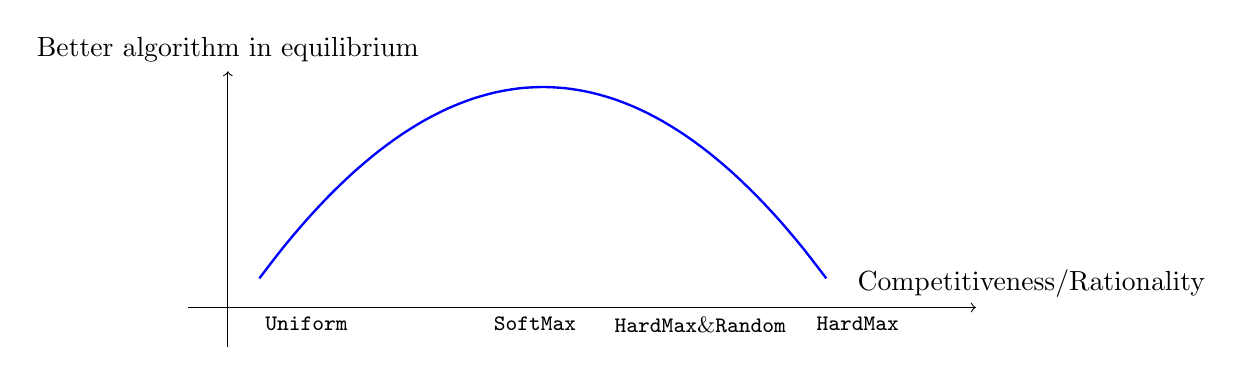
\begin{tikzpicture}[scale=1]
      \draw[->] (-.5,0) -- (9.5,0) node[above] 
        {\qquad\qquad Competitiveness/Rationality};
      \draw[->] (0,-.5) -- (0,3) node[above] {Better algorithm in equilibrium};
      \draw[scale=0.8,domain=0.5:9.5,smooth,variable=\x,blue, line width=0.3mm] plot ({\x},{3.5 - 0.15*(\x - 5)^2});
     \node[below] at (1, 0) {\footnotesize \Uniform};
     \node[below] at (3.9, 0) {\footnotesize \SoftMaxRandom};
     \node[below] at (6, 0) {\footnotesize \HardMaxRandom};
     \node[below] at (8, 0) {\footnotesize \HardMax};
      % \draw[scale=0.5,domain=-3:3,smooth,variable=\y,red]  plot ({\y*\y},{\y});
 \end{tikzpicture}

\caption{The stylized inverted-U relationship in the ``main story".}
\label{fig:inverted-U2}
\end{center}
\end{figure}


\xhdr{Secondary story.}
Let us zoom in on the symmetric  \HardMaxRandom model. \asedit{Competitiveness and rationality within this model are controlled by the baseline probability $\eps_0 = \respF(- 1)$, which goes smoothly between the two extremes of \HardMax ($\eps_0=0$) and the uniform choice ($\eps_0=\tfrac12$). Smaller $\eps_0$ corresponds to increased rationality and increased competitiveness.} For clarity, we assume that principal's utility is the number of agents.

We consider the marginal utility of switching to a better algorithm. Suppose initially both principals use some algorithm \alg, and principal 1 ponders switching to another algorithm \alg' which BIR-dominates \alg. \asedit{We are interested in the marginal utility of this switch. Then:}

\begin{itemize}
\item $\eps_0 = 0$ (\HardMax):~~~~ the marginal utility can be negative if \alg is \DynGreedy.

\item $\eps_0$ near $0$:~~~~ only a small marginal utility can be guaranteed, as it may take a long time for $\alg'$ to ``catch up" with \alg, and hence less time to reap the benefits.

\item ``medium-range" $\eps_0$:~~~~ large marginal utility, as $\alg'$ learns fast and gets most agents.

\item $\eps_0$ near $\tfrac12$:~~~~ small marginal utility, as principal 1 gets most agents for free no matter what.
\end{itemize}
The familiar inverted-U shape is depicted in Figure~\ref{fig:inverted-U3}.



\begin{figure}
\begin{center}
\begin{tikzpicture}[scale=1]
      \draw[->] (-.5,0) -- (9.5,0) node[above]  {$\eps_0$};
      \draw[->] (0,-.5) -- (0,3) node[above] {marginal utility};
      \draw[scale=0.8,domain=0.5:9.5,smooth,variable=\x,blue, line width=0.3mm] plot ({\x},{3.5 - 0.15*(\x - 5)^2});
     \node[below] at (.6, 0) {\footnotesize \Uniform};
     \node[above] at (.5, 0) {\footnotesize 0};
     % \node[below] at (3.9, 0) {\footnotesize \SoftMaxRandom};
     % \node[below] at (6, 0) {\footnotesize \HardMaxRandom};
     \node[below] at (7.5,0) {\footnotesize \HardMax};
     \node[above] at (7.5, 0) {\footnotesize 1/2};
      % \draw[scale=0.5,domain=-3:3,smooth,variable=\y,red]  plot ({\y*\y},{\y});
 \end{tikzpicture}

\caption{The stylized inverted-U relationship from the ``secondary story"}
\label{fig:inverted-U3}
\end{center}
\end{figure}




%%% Local Variables:
%%% mode: latex
%%% TeX-master: "main"
%%% End:


\paragraph{Acknowledgment}{ The authors would like to thank Glen Weyl
  for discussions of related work in economics.  }


% Bibliography
% \bibliographystyle{ACM-Reference-Format}
 \bibliographystyle{plainnat}
\bibliography{bib-abbrv-short,bib-AGT,bib-bandits,bib-slivkins,bib-random,bib-ML}

\appendix

\section{Background on multi-armed bandits}
\label{app:examples}

\newcommand{\ExplorExploit}{\term{ExplorExploit}}
\newcommand{\PhasedExplorExploit}{\term{PhasedExplorExploit}}
\newcommand{\RandomDynGreedy}{\term{RandomDynGreedy}}
\newcommand{\SuccesiveElimination}{\term{SuccesiveElimination}}
\newcommand{\SuccesiveEliminationReset}{\term{SuccesiveEliminationReset}}

This appendix provides some pertinent background on multi-armed
bandits (\emph{MAB}). We discuss \BIR and monotonicity of several MAB algorithms, touching upon: \DynGreedy and \StaticGreedy (Section~\ref{sec:MAB-greedy}), ``naive" MAB algorithms that separate exploration and exploitation (Section~\ref{sec:MAB-naive}), and ``smart" MAB algorithms that combine exploration and exploitation (Section~\ref{sec:MAB-smart}).

As we do throughout the paper, we focus on MAB with i.i.d. rewards and a Bayesian prior; we call it \emph{Bayesian MAB} for brevity.


% For a given mean reward vector $\mu$, the $n$-th step instantaneous regret is
%\begin{align}
%\regret(n\mid\mu) &:= \max_{a\in A} \mu_a - \rew(n\mid\mu),\\
%\regretWC(n)    &:=  \sup_{\text{mean reward vectors $\mu$}} \; \BIR(n\mid \mu).
%\end{align}


\subsection{\DynGreedy and \StaticGreedy}
\label{sec:MAB-greedy}

We provide an example when \DynGreedy and \StaticGreedy have
constant \BIR, and prove monotonicity of \DynGreedy. For the
example, it suffices to consider \emph{deterministic rewards} (for
each action $a$, the realized reward is always equal to the mean
$\mu_a$) and \emph{independent priors} (according to the prior
$\priorMu$, random variables $\mu_1 \LDOTS \mu_K$ are mutually
independent) each of {\em full support}.

%\ascomment{This lemma is just one example. Can we argue that constant \BIR is typical/reasonable?}
%
%
%\begin{lemma}
%There is a problem instance of Bayesian MAB such that \StaticGreedy
%and \DynGreedy have (at least) a constant \BIR for all steps. The
%problem instance has two actions, independent priors, and
%deterministic rewards.
%\end{lemma}
%
%\begin{proof}
%To specify the problem instance, it remains to specify the marginal
%distributions mean rewards $\mu_1$ and $\mu_2$ according to the
%prior. We posit that $\mu_1$ is uniform on the interval $[0, 1]$,
%and $\mu_2$ is uniform on the interval $[\tfrac13,1]$.
%
%Note that
%    $\OPT := \E[\max_{a\in A} \mu_a] =(1/3)(2/3)+(2/3)(7/9)=20/27$.
%%\ascomment{The numbers seem wrong, given the below?}
%This holds since with
%probability $1/3$ we have $\mu_1\leq 1/3$ in which case clearly the
%better arm is 2 with $\E[\mu_2]=2/3$ and with probability $2/3$ we
%have both $\mu_1,\mu_2\in[1/3,1]$ and distributed uniformly each.
%
%\StaticGreedy always recommends action $2$. Since
%$\E[\mu_2]=\tfrac23$, \BIR is $2/27$ in all rounds.
%
%\DynGreedy recommends the first agent action $2$. If $\mu_2 > 2/3$
%For all the following agents it recommends action $2$. Otherwise, it
%recommends agent $2$ action $1$ and for all the following agents it
%recommends the better action. The expectation for agents $t\geq 3$
%is $(1/2)(5/6)+(1/2)((1/2)(1/2)+(1/2)(5/9))=49/72$ and has
%instantaneous regret $13/216$.
%\end{proof}

The following claim is immediate from the definition of the CDF
function
\begin{claim}
Assume independent priors. Let $F_i$ be the CDF of the mean reward
$\mu_i$ of action $a_i\in A$. Then, for any numbers
$z_2>z_1>\E[\mu_2]$ we have
    $\Pr[\text{$\mu_1\leq z_1$ and $\mu_2\geq z_2$}] = F_1(z_1)(1-F_2(z_2)) $.
\end{claim}

%\begin{lemma}
%Let $\priorMu$ be the prior of the means, and assume that it is
%independent for each action, where for arm $i$ it has a mean $
%\E[\mu_i]$ and CDF $F_i$. Then, for any $\E[\mu_2] < z_1<z_2$ we
%have that with probability $F_1(z_1)(1-F_2(z_2))$ that both
%$\mu_1\leq z_1$ and $z_2\leq \mu_2$.
%\end{lemma}

%\begin{corollary}
%Any problem instance of Bayesian MAB for two actions and independent
%priors which are full support and deterministic rewards, with
%constant probability \DynGreedy has a constant \BIR for all steps.
%\end{corollary}


We can now draw an immediate corollary of the above claim

\begin{corollary}
Consider any problem instance of Bayesian MAB with two actions and independent
priors which are full support. Then:
\begin{OneLiners}
\item[(a)] With constant probability, \StaticGreedy  has a constant \BIR for all steps.
\item[(b)] Assuming deterministic rewards, with
constant probability \DynGreedy has a constant \BIR for all steps.
\end{OneLiners}
\end{corollary}

\begin{remark}
A similar result holds for  rewards which are distributed as
Bernoulli random variables. In this case we consider accumulative
reward of an action as a random walk, and use a high probability
variation of the law of iterated logarithms. (Details omitted.)
\end{remark}


Next, we show that \DynGreedy is monotone.

\begin{lemma}\label{dgmono}
\DynGreedy is monotone, in the sense that $\rew(n)$ is non-decreasing.
Further, $\rew(n)$ is strictly increasing for every time step $n$ with $\Pr[a_n\neq a_{n+1}]>0$.
\end{lemma}

\begin{proof}
We prove by induction on $n$ that $\rew(n)\leq \rew(n+1)$ for
\DynGreedy. Let $a_n$ be the random variable recommended at time
$t$, then $\E[\mu_{a_n}| \mI_n ]=\rew(n)$. We can rewrite this as:
\[
\rew(n)=\E_{\mI_n}[\E_{r_n}[\mu_{a_n}|r_n,\mI_n]] =
\E_{\mI_{n+1}}[\mu_{a_n}|\mI_{n+1}]
\]
since $\mI_{n+1}=(\mI_n,r_n)$. At time $n+1$ \DynGreedy will select
an action $a_{n+1}$ such that:
\[
\rew(n+1)=\E[\mu_{a_{n+1}}|\mI_{n+1}]\geq \E[\mu_{a_n}
|\mI_n]=\rew(n)
\]
%
%Now after executing action $a_n$ and observing its reward $r_n$
%there are two possibilities. If $a_n$ is still the best action, then
%its expected reward given the information at time $n$ has not
%changed. On the other hand, if $a_n$ is not the best action anymore,
%then it implies that we recommend a better action. In such a case,
%we increase the expected reward. \ymcomment{need to make this
%formal}
which proves the monotonicity. In cases that $\Pr[a_n\neq
a_{n+1}]>0]$ we have a strict inequality, since with some
probability we select a better action then the realization of $a_n$.
\end{proof}


%%%%%%%%%%%%%%%%%%%%%%%

\subsection{``Naive" MAB algorithms that separate exploration and exploitation}
\label{sec:MAB-naive}


%\ascomment{Nicer to have $\BIR(n)\leq n^{-1/3}$.
%Explore-then-exploit does not have that! So, let's use phases of
%exponentially increasing duration.}

MAB algorithm \ExplorExploit$(m)$ initially explores each action
with $m$ agents and for the remaining $T-|A|m$ agents recommends the
action with the highest observed average. In the explore phase it
assigns a random permutation of the $mK$ recommendations.

\begin{lemma}
%Assume that rewards in the range $[0,1]$.
The \ExplorExploit$(T^{2/3}\log |A|/\delta)$ algorithm has, with
probability $1-\delta$, for any  $n\geq |A|T^{2/3}$ we have
\BIR$(n)=O(T^{-1/3})$. In addition, \ExplorExploit$(m)$ is monotone.
\end{lemma}

\begin{proof}
In the explore phase we we approximate for each action $a\in A$, the
value of $\mu_a$ by $\hat{\mu}_a$. Using the standard Chernoff
bounds we have that with probability $1-\delta$, for every action
$a\in A$ we have $|\mu_a -\hat{\mu}_a| \leq T^{-1/3}$.

Let $a^* = \arg\max_a \mu_a$ and $a^{ee}$ the action that
\ExplorExploit selects in the explore phase after the first
$|A|T^{2/3}$ agents. Since $\hat{\mu}_{a^*} \leq
\hat{\mu}_{a^{ee}}$, this implies that $\mu_{a^*} -
\mu_{a^{ee}}=O(T^{-1/3})$.

To show that \ExplorExploit$(m)$ is monotone, we need to show only
that $\rew(mK) \leq \rew(mK+1)$. This follows since for any $t< mK$
we have $\rew(t)=\rew(t+1)$, since the recommended action is
uniformly distributed for each time $t$. Also, for any $t\geq mK+1$
we have $\rew(t)=\rew(t+1)$ since we are recommending the same
exploration action. The proof that $\rew(mK) \leq \rew(mK+1)$ is the
same as for \DynGreedy in Lemma~\ref{dgmono}.
\end{proof}

We can also have a a phased version which we call
\PhasedExplorExploit$(m_t)$, where time is partition in to phases.
In phase $t$ we have $m_t$ agents and a random subset of $K$ explore
the actions (each action explored by a single agent) and the other
agents exploit. (This implies that we need that $m_t\geq K$ for all
$t$. We also assume that $m_t$ is monotone in $t$.)

\begin{lemma}
Consider the case that $K=2$ and the rewards of the actions are
Bernoulli r.v. with parameter $\mu_i$ and $\Delta=\mu_1-\mu_2$.
Algorithm \PhasedExplorExploit$(m_t)$ is monotone and for $m_t =
\sqrt{t}$ it has $\BIR(n)=O(n^{-1/3}+e^{-O(\Delta^2 n^{2/3})}))$. 
\end{lemma}

\begin{proof}
We first show that it is monotone. Recall that $\mu_1>\mu_2$. Let
$S_i=\sum_{j=1}^t r_{i,j}$ be the sum of the rewards of action $i$
up to phase $t$. We need to show that $\Pr[S_1>S_2]+ (1/2)
\Pr[S_1=S_2]$ is monotonically increasing in $t$. Consider the
random variable $Z=S_1-S_2$. At each phase it increases by $+1$ with
probability $\mu_1(1-\mu_2)$, decreases by $-1$ with probability
$(1-\mu_1)\mu_2$ and otherwise does not change.

Consider the values of $Z$ up to phase $t$. We really care only
about the probability that is shifted from positive to negative and
vice versa.

First, consider the probability that $Z=0$. We can partition it to
$S_1=S_2=r$ events, and let $p(r,r)$ be the probability of this
event. For each such event, we have $p(r,r)\mu_1$ moved to $Z=+1$
and $p(r,r)\mu_2$ moved to $Z=-1$. Since $\mu_1>\mu_2$ we have that
$p(r,r)\mu_1\geq p(r,r)\mu_2$ (note that $p(r,r)$ might be zero, so
we do not have a strict inequality).

Second, consider the probability that $Z=+1$ or $Z=-1$. We can
partition it to $S_1=r+1;S_2=r$ and $S_1=r;S_2=r+1$ events, and let
$p(r+1,r)$ and $p(r,r+1)$ be the probabilities of those events.
%
It is not hard to see that $p(r+1,r)\mu_2=p(r,r+1)\mu_1$.
%
This implies that the probability mass moved from $Z=+1$ to $Z=0$ is
identical to that moved from $Z=-1$ to $Z=0$.

We have showed that $\Pr[S_1>S_2]+ (1/2) \Pr[S_1=S_2]$ and therefore
the expected valued of the exploit action is non-decreasing. Since
we have that the size of the phases are increasing, the $\BIR$ is
strictly increasing between phases and identical within each phase.

We now analyze the $\BIR$ regret. Note that agent $n$ is in phase
$O(n^{2/3})$ and the length of his phase is $O(n^{1/3})$. The $\BIR$
has two parts. The first is due to the exploration, which is at most
$O(n^{-1/3})$. The second is due to the probability that we exploit
the wrong action. This happens with probability $\Pr[S_1<S_2]+ (1/2)
\Pr[S_1=S_2]$ which we can bound using a Chernoff bound by
$e^{-O(\Delta^2n^{2/3})}$, since we explored each action
$O(n^{2/3})$ times.
\end{proof}

\begin{remark}
Actually we have a tradeoff depending on the parameter $m_t$ between
the regret due to exploration and exploitation. (Note that the
monotonicity is always guarantee assuming $m_t$ is monotone.) If we
can set that $m_t = 2^t$ then at time $n$ we have $2/ n$ probability
of an exploit action. For the explore action we are in phase $\log
n$ so the probability of a sub-optimal explore action is
$n^{-O(\Delta^{-2})}$. This should give us
$\BIR(n)=O(n^{-O(\Delta^{-2})})$.
\end{remark}


%MAB algorithm \RandomDynGreedy$(q_t)$for agent $t$ with probability
%$q_t$ selects a random action from $A$ and with probability $1-q_t$
%recommends the best action according to the current posterior
%(similar to \DynGreedy).
%\begin{lemma}
%%Assume that rewards in the range $[0,1]$.
%The algorithm \RandomDynGreedy$(q_t)$, where $q_t=t^{-1/3}$, has,
%with probability $1-\delta$, \BIR$(n)=O(K^{1/2}n^{-1/3}\log
%(K/\delta))$.
%\end{lemma}
%
%\begin{proof}
%At time $n$ we have that with probability $1-\delta/(2K)$, each
%action $a\in A$ was selected at least $n_a=\Theta(n^{2/3}/K)$ times.
%%
%This implies that with probability $1-\delta/(2K)$, for each $a$ we
%have $|\hat{\mu}_a-\mu_a|\leq K^{1/2}n^{-1/3}\log((2K)/\delta)$.
%%
%Therefore, the \BIR is $O(K^{1/2}n^{-1/3}\log((K)/\delta))$
%\end{proof}

%\ascomment{Add: can we modify Phased Explore-then-exploit to make it
%monotone? Perhaps choose exploration rounds u.a.r. within the
%phase?}

%
%\begin{lemma}
%\ExplorExploit$(m)$ is monotone
%\end{lemma}
%
%\begin{proof}
%We need to consider only time $m'=|A|m+1$. For any $n<m'$, we
%clearly have $\rew(n)=\rew(1)$.
%
%Consider two actions $a_1,a_2\in A$, such that $\mu_{a_1} \geq
%\mu_{a_2}$. We claim that the probability that $a_1$ is selected at
%time $m$ to be the exploit action is larger than the probability
%that $a_2$ is selected. This follows since $\hat{\mu}_{a_1}$
%stochastically dominates $\hat{\mu}_{a_2}$, which implies that for
%any threshold $\theta$ we have $\Pr[\hat{\mu}_{a_1}\geq\theta]\geq
%\Pr[\hat{\mu}_{a_2}\geq\theta]$.
%
%After the elimination we consider the expected reward of the
%selected action $\sum_{i\in A} \mu_i q_i$, where $q_i$ is the
%probability that action $i$ was selected for the exploit phase. We
%have that $q_i \geq q_{i+1}$, from the stochastic dominance.
%
%The sum $\sum_{i\in A} \mu_i q_i$ with $q_i \geq q_{i+1}$ and
%$\sum_i q_i=1$ is minimized by setting $q_i=1/|A|$. (We can see that
%if there are $q_i\neq 1/|A|$, then there are two $q_{i}> q_{i+1}$,
%and one can see that setting both to $(q_{i}+ q_{i+1})/2$ decreases
%the value.) Therefore we have that the $\rew(m')\geq\rew(m'-1)$.
%\end{proof}


\subsection{``Smart" MAB algorithms that combine exploration and exploitation}
\label{sec:MAB-smart}


%MAB algorithm \SuccesiveElimination holds a set of action
%$A_s\subset A$ which are called {\em surviving actions} and for
%agent $t$ selects a random action from $A_s$. Let $n_{i,t}$ be the
%number of times action $i$ has been selected up to time $t$, and
%$\hat{\mu}_{i,t}$ be the average of the rewards of action $i$ up to
%time $t$ and $\hat{\mu}^*=\max_i \hat{\mu}_{i,t}$. We eliminate
%action $i$ at time $t$, i.e., delete it from $A_s$, if
%$\hat{\mu}_t^*-\hat{\mu}_{i,t} > \log(T/\delta)/\sqrt{n/K}$.
%
%\begin{lemma}
%Assume that the prior is independent and if $\mu_i\geq \mu_j$ then
%$r_i$ stochastically dominates $r_j$.
%%
%The algorithm \SuccesiveElimination, has, with probability
%$1-\delta$, \BIR$(n)=O(\log(T/\delta)/\sqrt{n/K})$.
%\end{lemma}

%\begin{proof}
%Let the best action be $a^*=\arg\max_a \mu_a$. With probability
%$1-\delta$ at any time $n$ we have that for any action $i\in A_s$
%that $|\hat{\mu}_i -\mu_i|\leq \log(T/\delta)/\sqrt{n/K}$, and
%$a^*\in A_s$. This implies that any action $a$ such
%$\mu_{a^*}-\mu_{a}> 3\log(T/\delta)/\sqrt{n/K}$ is eliminated.
%Therefore, any action in $A_s$ has \BIR$(n)$ of at most
%$O(\log(T/\delta)/\sqrt{n/K})$. \ymcomment{should we get the
%constant right?}
%\end{proof}




%\ascomment{Add: Successive Elimination is monotone (or a simple
%modification thereof).}
%
%\begin{lemma}
%\SuccesiveElimination is monotone
%\end{lemma}
%
%\begin{proof}
%We will first show that for any two actions $a_1,a_2\in A$ that if
%$\mu_{a_1} \geq \mu_{a_2}$ then at any time $t$ we have that the
%probability that $a_1$ is eliminated is smaller than the probability
%that $a_2$ is eliminated, i.e., $\Pr[a_1 \not\in A_{s,t+1}| a_1\in
%A_{s,t} ]\geq \Pr[ a_2 \not\in A_{s,t+1}| a_2\in A_{s,t}]$.
%
%We first show that given this statement, the lemma holds and
%\SuccesiveElimination is monotone. Consider $\rew(t)$ versus
%$\rew(t+1)$. If the elimination probabilities would have been
%identical then we would have $\rew(t)=\rew(t+1)$. Consider the top
%two actions, and consider the elimination process in two phases,
%firs we eliminate both with the same probability, and hence the
%reward is unchanged, and then we eliminate only the second, which
%implies that we increase the the reward. The claim about the
%elimination probabilities rules out the case that the elimination
%probability of the best action is higher than then of the the second
%best. Therefore, overall the reward can only increase.
%
%
%We now need to prove the claim. Since $\mu_{a_1}\geq \mu_{a_2}$ and
%they use the same parametric family $\psi_a(\cdot)$ then
%$\hat{\mu}_{a_1}$ stochastically dominates $\hat{\mu}_{a_2}$. We
%actually need to show that $\hat{\mu}_{a_1}$ stochastically
%dominates $\hat{\mu}_{a_2}$ given that $a_1,a_2\in A_{s,t}$. If this
%holds, then the claim about the elimination would be immediate,
%since for any threshold $\theta$ we have $\Pr[\hat{\mu}_{a_1,t} <
%\theta |a_1\in A_{s,t}] \leq \Pr[\hat{\mu}_{a_2,t} < \theta |a_2\in
%A_{s,t}] $. By setting $\theta=\hat{\mu}^*-
%\log(T/\delta)/\sqrt{n/K}$ we derive the lemma.
%
%We now need to prove the claim. We first show that
%$\E[\hat{\mu}_{a_1}-\hat{\mu}_{a_2} | a_1,a_2\in A_s]\geq 0$ which
%is equivalent to $\E[\hat{\mu}_{a_1}-\hat{\mu}_{a_2} |
%\hat{\mu}_{a_1},\hat{\mu}_{a_2}\geq \hat{\mu}^*-\theta]\geq 0$ where
%$\theta$ is the threshold used in \SuccesiveElimination. Since
%action $a_1$ has a high expectation than $a_2$ it holds (at least
%for Bernoulli r.v.).
%
%
%[[OLD]]
%
% Clearly, for any actions $a\in A$ we have that $\Pr[a \in
%A_s]$ decreases with time. In addition, we have that with
%probability $1-\delta$ for every time $t$ we have $a^*\in A_s$.
%
%If $\mu_{a_1} \geq \mu_{a_2}$ then at any time $t$ we have
%$\Pr[a_1\in A_s]\geq \Pr[a_2\in A_s]$.
%
%
%We probably need to show that if $\mu_{a_1} \geq \mu_{a_2}$ then at
%any time $t$ we have that the probability that $a_1$ is eliminated
%is smaller than the probability that $a_2$ is eliminated, i.e.,
%$\Pr[a_1\in A_{s,t}, a_1 \not\in A_{s,t+1}]\geq \Pr[a_2\in A_s, a_2
%\not\in A_{s,t+1}]$.
%\end{proof}




%\ymcomment{Here is a simple modification of Successive-Elimination}



MAB algorithm \SuccesiveEliminationReset works as follows. It keeps
a set of surviving actions $A_s\subseteq A$, where initially
$A_s=A$. The agents are partition into phases, where each phase is a
random permutation of the non-eliminated actions.
% Initially, we select actions at random. Let $n_{i,t}$
%be the number of times action $i$ has been selected up to time $t$,
Let $\hat{\mu}_{i,t}$ be the average of the rewards of action $i$ up
to phase $t$ and $\hat{\mu}^*=\max_i \hat{\mu}_{i,t}$. We eliminate
action $i$ at the end of phase $t$, i.e., delete it from $A_s$, if
$\hat{\mu}_t^*-\hat{\mu}_{i,t} > \log(T/\delta)/\sqrt{t}$.
%So far identical to \SuccesiveElimination, the difference is how we
%continue after elimination.
In \SuccesiveEliminationReset we simply reset the algorithm with
$A=A_s-A_{e,t}$, where $A_{e,t}$ is the set of eliminated actions
after phase $t$. Namely, we restart $\hat{\mu}_{i,t}$ and ignore the
old rewards before the elimination.

\begin{lemma}
%
The algorithm \SuccesiveEliminationReset, has, with probability
$1-\delta$, \BIR$(n)=O(\log(T/\delta)/\sqrt{n/K})$.
\end{lemma}

\begin{proof}
Let the best action be $a^*=\arg\max_a \mu_a$. With probability
$1-\delta$ at any time $n$ we have that for any action $i\in A_s$
that $|\hat{\mu}_i -\mu_i|\leq \log(T/\delta)/\sqrt{n/K}$, and
$a^*\in A_s$. This implies that any action $a$ such
$\mu_{a^*}-\mu_{a}> 3\log(T/\delta)/\sqrt{n/K}$ is eliminated.
Therefore, any action in $A_s$ has \BIR$(n)$ of at most
$6\log(T/\delta)/\sqrt{n/K}$.
\end{proof}

\begin{lemma}
Assume that if $\mu_i\geq \mu_j$ then the rewards $r_i$
stochastically dominates the rewards $r_j$.
%
Then, \SuccesiveEliminationReset is monotone
\end{lemma}

\begin{proof}
Consider the first time $T$ an action is eliminated, and let
$T=\tau$ be a realized value of $T$. Then, clearly for $n<\tau$ we
have $\rew(n)=\rew(1)$ .

Consider two actions $a_1,a_2\in A$, such that $\mu_{a_1} \geq
\mu_{a_2}$. At time $T=\tau$, the probability that  $a_1$ is
eliminated is smaller than the probability that $a_2$ is eliminated.
This follows since $\hat{\mu}_{a_1}$ stochastically dominates
$\hat{\mu}_{a_2}$, which implies that for any threshold $\theta$ we
have $\Pr[\hat{\mu}_{a_1}\geq\theta]\geq
\Pr[\hat{\mu}_{a_2}\geq\theta]$.

After the elimination we consider the expected reward of the
eliminated action $\sum_{i\in A} \mu_i q_i$, where $q_i$ is the
probability that action $i$ was eliminated in time $T=\tau$. We have
that $q_i \leq q_{i+1}$, from the probabilities of elimination.

The sum $\sum_{i\in A} \mu_i q_i$ with $q_i \leq q_{i+1}$ and
$\sum_i q_i=1$ is maximized by setting $q_i=1/|A|$. (We can see that
if there are $q_i\neq 1/|A|$, then there are two $q_{i}< q_{i+1}$,
and one can see that setting both to $(q_{i}+ q_{i+1})/2$ increases
the value.) Therefore we have that the $\rew(\tau)\geq\rew(\tau-1)$.

Now we can continue by induction. For the induction, we can show the
property for {\em any} remaining set of at most $k-1$ actions. The
main issue is that \SuccesiveEliminationReset restarts from scratch,
so we can use induction.
\end{proof}







\end{document} 